%%%%%%%%%%%%%%%%%%%%%%%%%%%%%%%%%%%%%%%%%
% Arsclassica Article
% LaTeX Template
% Version 1.1 (1/8/17)
%
% This template has been downloaded from:
% http://www.LaTeXTemplates.com
%
% Original author:
% Lorenzo Pantieri (http://www.lorenzopantieri.net) with extensive modifications by:
% Vel (vel@latextemplates.com)
%
% License:
% CC BY-NC-SA 3.0 (http://creativecommons.org/licenses/by-nc-sa/3.0/)
%
%%%%%%%%%%%%%%%%%%%%%%%%%%%%%%%%%%%%%%%%%

%----------------------------------------------------------------------------------------
%	PACKAGES AND OTHER DOCUMENT CONFIGURATIONS
%----------------------------------------------------------------------------------------

\documentclass[
12pt, % Main document font size
a4paper, % Paper type, use 'letterpaper' for US Letter paper
oneside, % One page layout (no page indentation)
%twoside, % Two page layout (page indentation for binding and different headers)
headinclude,footinclude, % Extra spacing for the header and footer
BCOR5mm, % Binding correction
]{scrartcl}
%%%%%%%%%%%%%%%%%%%%%%%%%%%%%%%%%%%%%%%%%
% Arsclassica Article
% Structure Specification File
%
% This file has been downloaded from:
% http://www.LaTeXTemplates.com
%
% Original author:
% Lorenzo Pantieri (http://www.lorenzopantieri.net) with extensive modifications by:
% Vel (vel@latextemplates.com)
%
% License:
% CC BY-NC-SA 3.0 (http://creativecommons.org/licenses/by-nc-sa/3.0/)
%
%%%%%%%%%%%%%%%%%%%%%%%%%%%%%%%%%%%%%%%%%

%----------------------------------------------------------------------------------------
%	REQUIRED PACKAGES
%----------------------------------------------------------------------------------------

\usepackage[
nochapters, % Turn off chapters since this is an article
beramono, % Use the Bera Mono font for monospaced text (\texttt)
eulermath,% Use the Euler font for mathematics  eulermath
pdfspacing, % Makes use of pdftex’ letter spacing capabilities via the microtype package
dottedtoc % Dotted lines leading to the page numbers in the table of contents
]{classicthesis} % The layout is based on the Classic Thesis style

\usepackage{arsclassica} % Modifies the Classic Thesis package

\usepackage[T1]{fontenc} % Use 8-bit encoding that has 256 glyphs

\usepackage[utf8]{inputenc} % Required for including letters with accents

\usepackage{graphicx} % Required for including images
\graphicspath{{Figures/}} % Set the default folder for images

\usepackage{enumitem} % Required for manipulating the whitespace between and within lists

\usepackage{lipsum} % Used for inserting dummy 'Lorem ipsum' text into the template

\usepackage{subfig} % Required for creating figures with multiple parts (subfigures)

\usepackage{amsmath,amssymb,amsthm} % For including math equations, theorems, symbols, etc

\usepackage{varioref} % More descriptive referencing

%----------------------------------------------------------------------------------------
%	THEOREM STYLES
%---------------------------------------------------------------------------------------

\theoremstyle{definition} % Define theorem styles here based on the definition style (used for definitions and examples)
\newtheorem{definition}{Definition}

\theoremstyle{plain} % Define theorem styles here based on the plain style (used for theorems, lemmas, propositions)
\newtheorem{theorem}{Theorem}

\theoremstyle{remark} % Define theorem styles here based on the remark style (used for remarks and notes)

%----------------------------------------------------------------------------------------
%	HYPERLINKS
%---------------------------------------------------------------------------------------

\hypersetup{
%draft, % Uncomment to remove all links (useful for printing in black and white)
colorlinks=true, breaklinks=true, bookmarks=true,bookmarksnumbered,
urlcolor=webbrown, linkcolor=RoyalBlue, citecolor=webgreen, % Link colors
pdftitle={}, % PDF title
pdfauthor={\textcopyright}, % PDF Author
pdfsubject={}, % PDF Subject
pdfkeywords={}, % PDF Keywords
pdfcreator={pdfLaTeX}, % PDF Creator
pdfproducer={LaTeX with hyperref and ClassicThesis} % PDF producer
}  % Include the structure.tex file which specified the document structure and layout
% Specify custom hyphenation points in words with dashes where you would like hyphenation to occur, or alternatively, don't put any dashes in a word to stop hyphenation altogether

%----------------------------------------------------------------------------------------
%	TITLE AND AUTHOR(S)
%----------------------------------------------------------------------------------------

\title{{A summary of some mainstream spatial statistical methods for large datasets}} % The article title \normalfont\spacedallcaps

%\subtitle{Subtitle} % Uncomment to display a subtitle
\author{{Yewen Chen}} %\spacedlowsmallcaps The article author(s) - author affiliations need to be specified in the AUTHOR AFFILIATIONS block

\date{\normalsize{October 13, 2020}}
 % An optional date to appear under the author(s)

%----------------------------------------------------------------------------------------
\usepackage[margin=0.8in]{geometry}
\usepackage{tgbonum}
\usepackage{amsmath}
\usepackage{natbib}
\usepackage{float}
\usepackage{algorithm}
\usepackage{algpseudocode}
\usepackage{color}
\usepackage{fancyvrb}
\usepackage{relsize}
\usepackage{hyperref}
\usepackage{url}
\usepackage{bbm}
\hypersetup{
    colorlinks=true,
    linkcolor=blue,
    filecolor=magenta,
    urlcolor=cyan,
}

\urlstyle{same}
\newcommand{\VerbBar}{|}
\newcommand{\VERB}{\Verb[commandchars=\\\{\}]}
\DefineVerbatimEnvironment{Highlighting}{Verbatim}{commandchars=\\\{\}}
% Add ',fontsize=\small' for more characters per line
\usepackage{framed}
\definecolor{shadecolor}{RGB}{248,248,248}
\newenvironment{Shaded}{\begin{snugshade}}{\end{snugshade}}
\newcommand{\AlertTok}[1]{\textcolor[rgb]{0.94,0.16,0.16}{#1}}
\newcommand{\AnnotationTok}[1]{\textcolor[rgb]{0.56,0.35,0.01}{\textbf{\textit{#1}}}}
\newcommand{\AttributeTok}[1]{\textcolor[rgb]{0.77,0.63,0.00}{#1}}
\newcommand{\BaseNTok}[1]{\textcolor[rgb]{0.00,0.00,0.81}{#1}}
\newcommand{\BuiltInTok}[1]{#1}
\newcommand{\CharTok}[1]{\textcolor[rgb]{0.31,0.60,0.02}{#1}}
\newcommand{\CommentTok}[1]{\textcolor[rgb]{0.56,0.35,0.01}{\textit{#1}}}

\newcommand{\DataTypeTok}[1]{\textcolor[rgb]{0.13,0.29,0.53}{#1}}
\newcommand{\DecValTok}[1]{\textcolor[rgb]{0.00,0.00,0.81}{#1}}
\newcommand{\DocumentationTok}[1]{\textcolor[rgb]{0.56,0.35,0.01}{\textbf{\textit{#1}}}}
\newcommand{\ErrorTok}[1]{\textcolor[rgb]{0.64,0.00,0.00}{\textbf{#1}}}

\newcommand{\FunctionTok}[1]{\textcolor[rgb]{0.00,0.00,0.00}{#1}}
\newcommand{\ImportTok}[1]{#1}
\newcommand{\InformationTok}[1]{\textcolor[rgb]{0.56,0.35,0.01}{\textbf{\textit{#1}}}}
\newcommand{\KeywordTok}[1]{\textcolor[rgb]{0.13,0.29,0.53}{\textbf{#1}}}
\newcommand{\NormalTok}[1]{#1}
\newcommand{\OperatorTok}[1]{\textcolor[rgb]{0.81,0.36,0.00}{\textbf{#1}}}
\newcommand{\OtherTok}[1]{\textcolor[rgb]{0.56,0.35,0.01}{#1}}
\newcommand{\PreprocessorTok}[1]{\textcolor[rgb]{0.56,0.35,0.01}{\textit{#1}}}
\newcommand{\RegionMarkerTok}[1]{#1}
\newcommand{\SpecialCharTok}[1]{\textcolor[rgb]{0.00,0.00,0.00}{#1}}
\newcommand{\SpecialStringTok}[1]{\textcolor[rgb]{0.31,0.60,0.02}{#1}}
\newcommand{\StringTok}[1]{\textcolor[rgb]{0.31,0.60,0.02}{#1}}
\newcommand{\VariableTok}[1]{\textcolor[rgb]{0.00,0.00,0.00}{#1}}
\newcommand{\VerbatimStringTok}[1]{\textcolor[rgb]{0.31,0.60,0.02}{#1}}
\newcommand{\WarningTok}[1]{\textcolor[rgb]{0.56,0.35,0.01}{\textbf{\textit{#1}}}}

\begin{document}
\renewcommand{\UrlFont}{\small\tt}
\bibliographystyle{abbrvnat}
\setlength{\abovecaptionskip}{0pt}
\setlength{\belowcaptionskip}{10pt}
%----------------------------------------------------------------------------------------
%	HEADERS
%----------------------------------------------------------------------------------------
\renewcommand{\algorithmicrequire}{\textbf{Input:}}  % Use Input in the format of Algorithm
\renewcommand{\algorithmicensure}{\textbf{Update step:}} % Use Output in the format of Algorithm
\renewcommand{\sectionmark}[1]{\markright{\spacedlowsmallcaps{#1}}} % The header for all pages (oneside) or for even pages (twoside)
%\renewcommand{\subsectionmark}[1]{\markright{\thesubsection~#1}} % Uncomment when using the twoside option - this modifies the header on odd pages
\lehead{\mbox{\llap{\small\thepage\kern1em\color{halfgray} \vline}\color{halfgray}\hspace{0.5em}\rightmark\hfil}} % The header style

\pagestyle{scrheadings} % Enable the headers specified in this block

%----------------------------------------------------------------------------------------
%	TABLE OF CONTENTS & LISTS OF FIGURES AND TABLES
%----------------------------------------------------------------------------------------

\maketitle % Print the title/author/date block

\setcounter{tocdepth}{4} % Set the depth of the table of contents to show sections and subsections only

\tableofcontents % Print the table of contents

\listoffigures % Print the list of figures

\listoftables % Print the list of tables

%----------------------------------------------------------------------------------------
%	ABSTRACT
%----------------------------------------------------------------------------------------
\newpage
\section{Gaussian random field and its challenge}
Gaussian spatial processes has been popular for decades in spatial data contexts like geostatistics where they are known as kriging, and in computer experiments where they are deployed as surrogate models or emulators. More recently, they have become a popular prediction engine in the machine learning literature. The reasons are many, but the most important are probably that: the Gaussian structure affords a large degree of analytic capability not enjoyed by other general-purpose approaches to nonparametric nonlinear modeling; and because they perform well in out-of-sample tests.

Assume there is a response or dependent variable $Y(s)$ at a generic location $s \in \boldsymbol{D} \subset \mathcal{R}^2$ along with a $p \times 1$ vector of spatially referenced predictors $\boldsymbol{X}(s)$. A spatial regression model has the form
\begin{equation}
\begin{aligned}
y(s) = \boldsymbol{\beta}\boldsymbol{X}(s) + w(s) + \epsilon(s)
\end{aligned} \label{model}
\end{equation}
where $\boldsymbol{\beta}$ is the vector of regression coefficients. The residual from the regression is decomposed into two independent parts: a spatial process, $w(s)$, modelling spatial association, and an independent process, $\epsilon(s)$, also known as the nugget effect, modelling measurement error. The spatial process $w(s)$ in (\ref{model}) is often referred to as spatial random effects, capturing the effect of unmeasured or unobserved covariates with spatial pattern.

The nugget effect $\epsilon(s)$ is often assumed to follow a normal distribution with variance $\tau^2$ for every location $s$.
The most common specification for $w(s)$ is $w(s) \sim GP(0, \boldsymbol{C}(\cdot, \cdot))$, a zero-mean Gaussian process with a valid covariance function $\boldsymbol{C}(s, s^\prime)$. It is often reasonable to assume a constant process variance and thus we specify \
$\boldsymbol{C}(s, s^\prime) = \sigma^2 \rho (s, s^\prime; \boldsymbol{\theta})$, where $\rho (s, s^\prime; \boldsymbol{\theta})$ is a correlation function and $\boldsymbol{\theta}$ is a vector of correlation parameters which needs to be estimated from a finite number of observations, $\boldsymbol{Y} = \left(y(s_1). \cdots, y(s_n)\right)^\prime$.

According to the above assumptions, $y(s)$ follows a spatial Gaussian process, and thus we have the log-likelihood function for $\Theta = (\boldsymbol{\beta}, \tau^2, \sigma^2, \boldsymbol{\theta}):$
\begin{equation}
\begin{aligned}
l(\Theta) \propto  - \frac{1}{2}\log |\boldsymbol{\Sigma}| - \frac{1}{2}\left(\boldsymbol{y} - \boldsymbol{\beta}\boldsymbol{X}\right)^\prime \boldsymbol{\Sigma}^{- 1}\left(\boldsymbol{y} - \boldsymbol{\beta}\boldsymbol{X}\right)
\end{aligned} \label{loglik}
\end{equation}
where $\boldsymbol{\Sigma} = \boldsymbol{C} + \tau^2\boldsymbol{I}.$ From Bayesian point of view, the posterior distributions of the parameter $\Theta$ are derived by
\begin{equation}
\begin{aligned}
p(\Theta|\boldsymbol{y}) \propto \overbrace{p(\boldsymbol{y}|\boldsymbol{w}, \boldsymbol{\beta}, \tau^2)}^{\texttt{data model}} \underbrace{p(\boldsymbol{w}|\theta)}_{\texttt{process model}}\pi\left(\Theta\right)
\end{aligned} \label{posloglik}
\end{equation}
From (\ref{posloglik}), the real challenge lies in the process model $p(\boldsymbol{w}|\theta)$ rather than the data model $p(\boldsymbol{y}|\boldsymbol{w}, \boldsymbol{\beta}, \tau^2)$ in terms of computation, that is because covariance matrix of the process model, typically, is dense while it is just a diagonal matrix for the data model. Therefore, we turn to study $\boldsymbol{w}$ in the process model.

As we all know, the best linear unbiased prediction (BLUP) $\hat{w}(s_0)$ at an unobserved location $s_0$ can be obtained by the \textbf{Kriging
equation}:
\begin{equation}
\begin{aligned}
\hat{w}(s_0) = \boldsymbol{c}_{s_0}^\prime\boldsymbol{C}^{- 1}\boldsymbol{w}
\end{aligned} \label{Kriging}
\end{equation}
where $\boldsymbol{c}_{s_0} = \left(\boldsymbol{C}(s_0, s_1), \dots, \boldsymbol{C}(s_0, s_n)\right)^\prime$.

However, with large or massive data (e.g., $n = 10^5$ or more), direct implementation of these statistical process, including parameter etimation by (\ref{loglik}) or (\ref{posloglik}) and interpolation by (\ref{Kriging}), becomes computationally prohibitive, since evaluation of the likelihood of the process model in (\ref{posloglik}) (or the likelihood in (\ref{loglik})) or solution of the Kriging equation (\ref{Kriging}) involve the Cholesky factorization of an $n \times n$ covariance matrix for data of size $n$, which requires $O(n^3)$ operations and $O(n^2)$ memory in general (see, e.g., \href{https://chenyw68.github.io/Literature/[2012]Advances and Challenges in Space-time Modelling of Natural Events.pdf}{\cite{porcu2012advances}}, \href{https://chenyw68.github.io/Literature/[2012]A full scale approximation of covariance functions for large spatial data sets.pdf}{\cite{sang2012full}}, \href{https://chenyw68.github.io/Literature/[2018]A case study competition among methods for analyzing large spatial data.pdf}{\cite{heaton2019case}}, \href{https://chenyw68.github.io/Literature/[2020]A Fused Gaussian Process Model for Very Large Spatial Data.pdf}{\cite{ma2020fused}}).

\section{Several approaches to overcome the computational problem}
The \textcolor[rgb]{0.50,0.50,0.50}{approximation of the likelihood in either the spatial or spectral domain} and the \textcolor[rgb]{0.50,0.50,0.50}{lower-dimensional representation} are fundamental solutions to overcome computational obstacles. These solutions focus on model development, the design of efficient and parallel algorithms, and the improvement and efficient use of modern computing platforms (e.g., Using \href{https://hpc.niasra.uow.edu.au/azm/Spatial_GPUs.html}{TensorFlow} and \href{https://github.com/cdeterman/gpuR}{GPU}).

\textbf{Developed models, official websites of scholars}:
\begin{itemize}
  \item [1)] Conditional distributions: \href{http://www.stat.uchicago.edu/~stein/}{Michael L. Stein} (The restricted likelihood, \href{https://chenyw68.github.io/Literature/[2004]Approximating likelihoods for large spatial data sets.pdf}{2004});
  \item [2)] Sparse covariance by tapering method: \href{http://user.math.uzh.ch/furrer/}{Reinhard Furrer}(\href{https://chenyw68.github.io/Literature/[2006]Covariance tapering for interpolation of large spatial datasets.pdf}{2006});
       \href{https://dnychka.github.io/}{Douglas Nychka} (bias correction, \href{https://chenyw68.github.io/Literature/[2008]Covariance Tapering for Likelihood Based Estimation in Large Spatial Data Sets.pdf}{2008}); \href{http://www.stat.uchicago.edu/~stein/}{Michael L. Stein} (Statistical Properties, \href{https://chenyw68.github.io/Literature/[2013]Statistical Properties of Covariance Tapers.pdf}{2013});
  \item [3)] Low-Rank methods: \href{https://niasra.uow.edu.au/cei/people/UOW202822.html}{Noel Cressie} (FRK, \href{https://chenyw68.github.io/L iterature/[2008]Fixed rank kriging for very large spatial data sets.pdf}{2008}),
  \href{https://ph.ucla.edu/faculty/banerjee}{Sudipto Banerjee} (Predictive process, \href{https://chenyw68.github.io/Literature/[2008]Gaussian predictive process models for large spatial data sets.pdf}{2008}); \href{https://sites.google.com/view/katzfuss/}{Matthias Katfuss} (multiresolution approximation where the basis functions are automatically chosen, \href{https://chenyw68.github.io/Literature/[2017]A Multi-Resolution Approximation for Massive Spatial Datasets.pdf}{2017});
  \item [4)] Sparse precision: \href{https://dnychka.github.io/}{Douglas Nychka} (lattice kriging, \href{https://chenyw68.github.io/Literature/[2015]A Multiresolution Gaussian Process Model for the Analysis of Large Spatial Datasets.pdf}{2015}) by basis-function;
   \href{https://www.maths.ed.ac.uk/~flindgre/}{Finn Lindgren} (GRMF Approximations, \href{https://chenyw68.github.io/Literature/[2011]An explicit link between GF and GMRFs the SPDE approach.pdf}{2011}) by SPDE;
   \href{http://abhidatta.com/}{Abhi Datta} (NNGP, \href{https://chenyw68.github.io/Literature/[2016]Hierarchical nearest-neighbor Gaussian process models for large geostatistical datasets.pdf}{2016a},
\href{https://chenyw68.github.io/Literature/[2016]On nearest neighbor Gaussian process models for massive spatial data.pdf}{2016b},
\href{https://chenyw68.github.io/Literature/[2016]Nonseparable dynamic NNGP models for large spatio-temporal data.pdf}{2016c},
\href{https://chenyw68.github.io/Literature/[2019]Efficient algorithms for bayesian nearest neighbor gaussian processes.pdf}{2019}) by conditional distributions;
  \item [5)] Spectral method: \href{https://scholar.google.com/citations?user=xPuzEj8AAAAJ&hl=zh-CN}{Montserrat Fuentes} and \href{http://guinness.cals.cornell.edu/}{Joe Guinness} (Circulant embedding, \href{https://chenyw68.github.io/Literature/[2017]Circulant Embedding of Approximate Covariances for Inference From Gaussian Data.pdf}{2017} and Periodic Embeddings,  \href{https://chenyw68.github.io/Literature/[2007]Approximate Likelihood for Large Irregularly Spaced Spatial Data.pdf}{2007},  \href{https://chenyw68.github.io/Literature/[2020]Spectral Density Estimation for Random Fields via Periodic Embeddings.pdf}{2019}).
  \item [6)] Discrete process convolutions. \href{https://scholar.google.com/citations?user=0FDdexMAAAAJ&hl=zh-CN}{Dave Higdon} (\href{https://chenyw68.github.io/Literature/[2002]Space and Space-Time Modeling Using Process Convolutions.pdf}{2002});
      \href{https://users.soe.ucsc.edu/~bruno/}{Bruno Sansó} (\href{https://chenyw68.github.io/Literature/[2009]A Spatio Temporal Model for Mean Anomaly and Trend Fields of North Atlantic Sea Surface Temperature.pdf}{2009}); \href{https://scholar.google.com/citations?user=qKdSQUsAAAAJ&hl=en}{Fra-ncky Fouedjio} (\href{https://chenyw68.github.io/Literature/[2016]A generalized convolution model and estimation for non-stationary random functions.pdf}{2016}).
  \item [7)] \href{https://chenyw68.github.io/Literature/[2016]laGP.pdf}{Local approximate Gaussian processes}:  \href{https://bobby.gramacy.com/research/}{Robert B. Gramacy}, \href{https://chenyw68.github.io/Literature/[2014]Local Gaussian Process Approximation for Large Computer Experiments.pdf}{\citep{gramacy2015local}};
  \item [8)] Vecchia’s approximation: \href{https://chenyw68.github.io/Literature/[2020]Vecchia laplace approximations of generalized gaussian processes.pdf}{\cite{zilber2019vecchia}}, \href{https://chenyw68.github.io/Literature/[2020]Vecchia Approximations of Gaussian-Process Predictions.pdf}{\cite{katzfuss2020vecchia}} and \href{https://chenyw68.github.io/Literature/[2020]Hierarchical sparse Cholesky decomposition with applications to spatio-temporal filtering.pdf}{\cite{jurek2020hierarchical}}.
\end{itemize}


\textbf{Developed algorithms and platforms, official websites of scholars}:
\begin{itemize}
  \item [1)] INLA: \href{https://cemse.kaust.edu.sa/bayescomp}{Haavard Rue}.
  \item [2)] Parallel algorithm: \href{https://sites.google.com/view/katzfuss/}{Matthias Katfuss}.
  \item [3)] TensorFlow: \href{https://niasra.uow.edu.au/cei/people/UOW202823.html}{Andrew Zammit-Mangion}.
\end{itemize}
\begin{table}[H]
	\caption{Application situations for different models}
\begin{tabular}{|l|c|c|c|}
\hline
{\bf Model} & {\bf non-stationary} & {\bf space-time} & {\bf multivariate data} \\
\hline
       FRK &  $\surd$    &   $\surd$         &     $\surd$       \\
\hline
Predictive process &   $\surd$     &    $\surd$   &  $\surd$          \\
\hline
       MRA &  $\surd$     &    $\surd$    &            \\
\hline
  Tapering &      &    $\surd$   &    $\surd$    \\
\hline
Spatial partitioning &            &            &            \\
\hline
LatticeKrig &   $\surd$     &   $\times$    &   $\times$    \\
\hline
      SPDE &   $\surd$    &    $\surd$   &    $\surd$  \\
\hline
      NNGP &   $\surd$    &    $\surd$    &   $\surd$         \\
\hline
Whittle’s approximation &   $\times$      &   $\times$    &    $\times$   \\
\hline
\end{tabular}
  \label{table:Scope}
\end{table}

The websites of other scholars: 1) \href{https://www.stat.missouri.edu/people/wikle}{Christopher K. Wikle}, 2)
\href{https://www.counterpointstat.com/bradleycarlin.html}{Bradley P. Carlin}, 4)
\href{https://cemse.kaust.edu.sa/stochproc}{David Bolin}, 5)
\href{https://gufaculty360.georgetown.edu/s/contact/00336000014SrlEAAS/jonathan-stroud}{Jonathan R. Stroud}, 6)
\href{https://www.bus.miami.edu/thought-leadership/faculty/management-science/guan.html}{YongTao Guan}, 7)
\href{http://www2.stat.duke.edu/~alan/}{Alan E. Gelfand}, 8)
\href{https://www.lancaster.ac.uk/staff/diggle/}{Peter J. Diggle}, 9)
\href{https://www.stat.tamu.edu/~huiyan/}{Huiyan  Sang}, 10)
\href{https://www.canr.msu.edu/people/andrew_o_finley}{Andrw Finley}, 11)
\href{https://mheaton.byu.edu/docs/research.html}{Matthew J. Heaton}, 12)
\href{https://www.kaust.edu.sa/en/study/faculty/ying-sun}{Ying Sun}, 13)
\href{https://scholar.google.com/citations?user=dbFZvbwAAAAJ&hl=en}{Furong Sun}, 14)
\href{https://sites.google.com/site/jonathanbradley28/}{Jonathan R. Bradley}.



\section{Likelihood approximations in the spectral domain}
\subsection{Whittle’s likelihood}

%: circulant embedding and periodic embeddings
%Likelihood approximations
%\textcolor[rgb]{1.00,0.00,1.00}{Comment:}
The spectral methods are computationally efficient by avoiding the calculation of determinants and can be easily adapted to model nonstationary processes as a mixture of independent stationary processes.

\href{https://chenyw68.github.io/Literature/[2007]Approximate Likelihood for Large Irregularly Spaced Spatial Data.pdf}{\cite{fuentes2007approximate}}, \href{https://chenyw68.github.io/Literature/[2020]Spectral Density Estimation for Random Fields via Periodic Embeddings.pdf}{\citep{guinness2019spectral}} and \href{https://chenyw68.github.io/Literature/[2017]Circulant Embedding of Approximate Covariances for Inference From Gaussian Data.pdf}{\citep{guinness2017circulant}} propose the use of small domain expansions and imputing data in a periodic fashion on the expanded lattice and  presented a version of Whittle’s approximation to the Gaussian negative log-likelihood by introducing a lattice process which can be used to deal with irregularly spaced data. Additional computational savings were obtained by truncating the spectral representation of the lattice process. The calculation requires $O(m \log_2 m + n)$ operations where $m$ is lattice size.

\textcolor[rgb]{1.00,0.00,1.00}{Comment:}
The flexibility of the spectral methods mentioned above are disputable for prediction problem respecting out of sample data, since the expanded lattice is pre-difined.
%\href{https://chenyw68.github.io/Literature/[2020]Bayesian Inference for Big Spatial Data Using Non-stationary Spectral Simulation.pdf}{\citep{yang2020bayesian}}

\section{Likelihood approximations in the spatial domain}
\subsection{Low rank methods}
\textcolor[rgb]{1.00,0.00,1.00}{Comment:}
The reduced rank based methods usually fail to accurately capture the local, small scale dependence structure (see \href{https://chenyw68.github.io/Literature/[2012]A full scale approximation of covariance functions for large spatial data sets.pdf}{\citep{sang2012full}}, \href{https://chenyw68.github.io/Literature/[2008]A modeling approach for large spatial datasets.pdf}{\citep{stein2008modeling}} and \href{https://chenyw68.github.io/Literature/[2009]Improving the performance of predictive process modeling for large datasets.pdf}{\citep{finley2009improving}}).
%The subsequent multiresolution (MR) methods (e.g.,  LatticeKrig, Multiresolution Approximations) compensates for this problem to some extent.
\subsubsection{\href{https://chenyw68.github.io/Literature/[2017]An R Package for Spatial and Spatio-Temporal Prediction with Large Datasets(FRK).pdf}{Fixed rank Kriging}}
FRK (\href{https://chenyw68.github.io/Literature/[2006]Spatial prediction for massive datasets.pdf}{\citep{cressie2006spatial}}, \href{https://chenyw68.github.io/Literature/[2008]Fixed rank kriging for very large spatial data sets.pdf}{\citep{cressie2008fixed}}) aims to approximate the spatial process $w(s)$ in (\ref{model}) by a linear combination of $K$ ($\ll n$) \textbf{multi-resolution bisquare} basis functions: \begin{equation}
\begin{aligned}
w(s) = \sum_{r = 1}^{R}\sum_{k = 1}^{K_r}h_{rk}(s)w_{rk}^{\star}
\end{aligned} \label{FRK}
\end{equation}
where $K = \sum_{r = 1}^{R}K_r$ and the coefficients $w^{\star}$ is an $K$-dimensional Gaussian vector with mean zero and exponential covariance  defined by some small basic areal units.
which ensures that all estimation and prediction equations only contain inverses of matrices of size $K \times K$.

\textcolor[rgb]{1.00,0.00,1.00}{Comment:}
Since covariance matrix for every resolutions is dense, that implies FRK can be challenging for large $K_r$.


\subsubsection{\href{https://chenyw68.github.io/Literature/[2015]spBayes for Large Spatio-Temporal Data Models.pdf}{Gaussian predictive processes} (\href{https://chenyw68.github.io/Literature/[2020]Bayesian spatially varying coefficient models in the spBayes R package.pdf}{GPP})}
With regard to the challenge of computational cost on covariance matrices, \href{https://chenyw68.github.io/Literature/[2008]Gaussian predictive process models for large spatial data sets.pdf}{\citet{banerjee2008gaussian}} proposed a class of models based on the idea of a spatial predictive process which is motivated by Kriging equation in (\ref{Kriging}). The predictive process projects the original process, $w(s)$ in (\ref{model}), onto a subspace generated by realizations of the original process at a specified set of locations (or knots), e.g.,  $s_1^{\star}, \cdots, s_K^{\star}, K \ll n$. The approach is in the same spirit as process modeling approaches using basis functions and kernel convolutions, that is, specifications which attempt to facilitate computations through lower dimensional process representations, i.e.
\begin{equation}
\begin{aligned}
w(s) = \boldsymbol{c}_{s}^\prime\boldsymbol{\Sigma}_{w^{\star}}^{-1}w_{rk}^{\star}
\end{aligned} \label{GPP}
\end{equation}
where $\boldsymbol{c}_{s} = \left(\boldsymbol{C}(s, s_1^{\star}), \dots, \boldsymbol{C}(s, s_K^{\star})\right)^\prime$, and then $\boldsymbol{c}_{s}^\prime\boldsymbol{\Sigma}_{w^{\star}}^{-1}$ plays the same role as $h$ in (\ref{FRK}), and thus can be regarded as some basis functions.

\textcolor[rgb]{1.00,0.00,1.00}{Comment:}
\begin{itemize}
 \item [1)]One advertised advantage of using the GPP approach as opposed to \href{https://chenyw68.github.io/Literature/[2017]FRK_intro.pdf}{FRK} or \href{https://chenyw68.github.io/Literature/[2014]LatticeKrig A multi-resolution spatial model for large data.pdf}{LatticeKrig} is that the GPP basis functions are completely determined by the choice of covariance function $C(\cdot, \cdot)$, and note that the subsequent \href{https://chenyw68.github.io/Literature/[2017]A Multi-Resolution Approximation for Massive Spatial Datasets.pdf}{Multiresolution approximations} is in step with GPP in this regard.
\item [2)]At the same time, however, when $C(\cdot, \cdot)$ is governed by unknown parameters (which is nearly always the case) the GPP basis functions need to be calculated iteratively rather than once as in FRK or LatticeKrig which will subsequently increase computation time.
\end{itemize}

\subsubsection{Multi-resolution approximations}
In contrast to FRK or LatticeKrig, the multi-resolution approximation (MRA) basis functions and the prior distribution of the corresponding weights $w_r^{\star}$ are chosen using the predictive-process approach to automatically adapt to any given covariance function $\boldsymbol{C}_r$, and so the MRA can adjust flexibly to a desired spatial smoothness and dependence structure. The MRA allows the number of basis functions to be approximately the same as the data by the two ways to do. The one is by increasing sparsity of the covariance matrices of the corresponding weights (achieved by tapering method, see  \href{https://chenyw68.github.io/Literature/[2017-formal]Parallel inference for massive distributed spatial data using low-rank models.pdf
}{\citep{katzfuss2017parallel}}), the other is by recursively partitioning the spatial domain (see \href{https://chenyw68.github.io/Literature/[2017]A Multi-Resolution Approximation for Massive Spatial Datasets.pdf}{\citep{katzfuss2017multi}}).

\textcolor[rgb]{1.00,0.00,1.00}{Comment:} Two obvious advantages of MRA are the ability to compute in parallel and capture spatial structure from very fine to very large scales.

%\href{https://chenyw68.github.io/Literature/[2012]Advances and Challenges in Space-time Modelling of Natural Events.pdf}{\citep{porcu2012advances}}

%\href{https://user.math.uzh.ch/furrer/software/KriSp/}{Tapering}
\subsection{Sparse covariance methods}
\subsubsection{\href{https://user.math.uzh.ch/furrer/software/KriSp/}{Tapering}}
Including \href{https://chenyw68.github.io/Literature/[2008]Covariance Tapering for Likelihood Based Estimation in Large Spatial Data Sets.pdf}{tapering for estimation} (e.g.,  approximation log-likelihood function by a tapered covariance. See \href{https://chenyw68.github.io/Literature/[2008]Covariance Tapering for Likelihood Based Estimation in Large Spatial Data Sets.pdf}{\cite{kaufman2008covariance}}) and \href{https://chenyw68.github.io/Literature/[2006]Covariance tapering for interpolation of large spatial datasets.pdf}{tapering for Kriging} (or for interpolation or for prediction, e.g.,  approximation Kriging equation by replacing the original covariance by a tapered version. See \href{https://chenyw68.github.io/Literature/[2006]Covariance tapering for interpolation of large spatial datasets.pdf}{\cite{furrer2006covariance}} and some R packages: \href{https://chenyw68.github.io/Literature/[2010]spam-A Sparse Matrix R Package with Emphasis on MCMC Methods for Gaussian Markov Random Fields.pdf}{spam}, 2010; \href{https://chenyw68.github.io/Literature/[2006]KriSp.pdff}{KriSp}, 2006; \href{https://chenyw68.github.io/Literature/[2020]fields.pdf}{fields}, 2017.

\textcolor[rgb]{1.00,0.00,1.00}{Comment:}
The covariance tapering has shown great computational gains, but it also has its own drawbacks.
\begin{itemize}
 \item [1)]The covariance tapering may not be effective in accounting for \textbf{spatial dependence with long range}.
 \item [2)]The accuracy of the tapering approximation for \textbf{nonstationary problems} remains an open question, and the application of tapering techniques to \textbf{multivariate random fields} (e.g.,  \href{https://chenyw68.github.io/Literature/[2015]Covariance tapering for multivariate Gaussian random fields estimation.pdf}{\citep{bevilacqua2016covariance}}) remains to be explored due to the lack of flexible compactly supported cross-covariance functions, see \href{https://chenyw68.github.io/Literature/[2012]Advances and Challenges in Space-time Modelling of Natural Events.pdf}{\citet{porcu2012advances}}.
\end{itemize}
\subsubsection{Spatial partitioning}
By dividing region $\boldsymbol{D}$ into $m$ disjoint subregions ($d = 1, 2, \cdots, m$),  and then the modeling approach based on spatial
partitioning is to again assume the model in (\ref{model2}) but take on the assumption of independence between observations across subregions, and then
\begin{equation}
\begin{aligned}
\boldsymbol{y}_d = \boldsymbol{\beta}\boldsymbol{X}_d + \boldsymbol{H}_d\boldsymbol{w} + \boldsymbol{\xi}_d + \boldsymbol{\epsilon}_d
\end{aligned} \label{model2}
\end{equation}
where $\boldsymbol{H}_d$ is a matrix of spatial basis function for subregions $d$.

\textcolor[rgb]{1.00,0.00,1.00}{Comment:}
\begin{itemize}
 \item [1)] Notice that, in (\ref{model2}) each subregion shares common $\boldsymbol{\beta}$ and $\boldsymbol{w}$ parameters which allows smoothing across subregions in spite of the independence assumption. Further, the assumption of independence across subregions effectively creates a block-diagonal structure for $\boldsymbol{\Sigma}$ and allows the likelihood to be computed in parallel (with one node per subregion), thereby facilitating computation.
 \item [2)] The key to implementing the spatial partitioning approach is the choice of partition and the literature is replete with various options.
  A priori methods to define the spatial
partitioning include partitioning the region into equal areas (\href{https://chenyw68.github.io/Literature/[2011]Covariance approximation for large multivariate spatial data sets.pdf}{\citep{sang2011covariance}}), partitioning based on centroid clustering (\href{https://chenyw68.github.io/Literature/[2005]Analyzing nonstationary spatial data using piecewise Gaussian processes.pdf}{\citep{kim2005analyzing}}), hierarchical clustering based on spatial gradients (\href{https://chenyw68.github.io/Literature/[2017]Nonstationary GP Models Using Spatial Hierarchical Clustering from Finite Differences.pdf}{\citep{heaton2017nonstationary}}). Alternatively, model-based approaches to spatial partitioning include treed regression(\href{https://chenyw68.github.io/Literature/[2014]Adaptive Bayesian Nonstationary Modeling for Large Spatial Datasets.pdf}{\citep{konomi2014adaptive}}) and mixture modeling (\href{https://chenyw68.github.io/Literature/[2014]A multivariate spatial mixture model for areal data.pdf}{\citet{neelon2014multivariate}}), but these approaches typically require more computation.
\end{itemize}


\subsection{Sparse precision methods}
The sparse precision methods focus on basis function and conditional likelihood.

\subsubsection{\href{https://chenyw68.github.io/Literature/[2020]LatticeKrigVignette.pdf}{LatticeKrig}}
LatticeKrig (LK, \href{https://chenyw68.github.io/Literature/[2015]A Multiresolution Gaussian Process Model for the Analysis of Large Spatial Datasets.pdf}{\citep{nychka2015multiresolution}}) uses nearly the same setup as is employed by FRK. Here is just a list of the differences:
%\textcolor[rgb]{1.00,0.00,1.00}{Comment:}
\begin{itemize}
 \item [1)] FRK uses families of \textbf{bisquare} basis functions allowing different resolutions that are organized on \textcolor[rgb]{0.50,0.50,0.50}{irregular} basic areal units (BAUs), and LK uses families of \textbf{radial} basis functions that are organized on \textcolor[rgb]{0.50,0.50,0.50}{regular} grids of increasing resolution.
 \item [2)] Covariance matrix, $\boldsymbol{\Sigma}_r$, of the coefficients $w_r^{\star}$ in (\ref{FRK}) is constrained by a exponential function, the exponential function is defined on the centroids of the BAUs. However, precision matrix, $\boldsymbol{Q}_r$, of the coefficients $w_r^{\star}$ in LK is constrained to a spatial autoregressive (SAR, defined on the regular lattice) model and forced to admit some sparse structures by following the ideas of \href{https://chenyw68.github.io/Literature/[2011]An explicit link between GF and GMRFs the SPDE approach.pdf}{\citet{lindgren2011explicit}}.
 \item [3)] Furthermore, because $\boldsymbol{Q}_r$ is sparse, \textbf{LK can set $K$ to be very large (e.g.,  $K > n$) without much additional computational cost}. However, the FRK does not achieve this effect.
\end{itemize}

\subsubsection{\href{http://www.r-inla.org/}{Gaussian Markov random field approximations by SPDE}}
\href{https://chenyw68.github.io/Literature/[2005]Gaussian markov random fields theory and applications.pdf}{\citet{rue2005gaussian}} rigorously suggest to approximate \textcolor[rgb]{0.50,0.50,0.50}{Gaussian random fields} through \textcolor[rgb]{0.50,0.50,0.50}{Markov fields} with a huge increase in speed for the simulations and demonstrated empirically that GMRFs could
closely approximate some commonly used covariance functions in geostatistics, and whereafter \href{https://chenyw68.github.io/Literature/[2011]An explicit link between GF and GMRFs the SPDE approach.pdf}{\citet{lindgren2011explicit}} show the construction of the corresponding GMRFs can be used to represent the Matérn field on a triangulated lattice (i.e., the finite element construction).

Similar to FRK or LatticeKrig, the spatial process $w(s)$ in model (\ref{model}) is represented by the basis function,  this method
use piecewise linear functions on a triangulation of the domain as basis functions $h(\cdot)$ in (\ref{FRK}), and then this yields sparse matrices $\boldsymbol{C}$ and $\boldsymbol{G}$ such that the appropriate precision matrix for the weights $\boldsymbol{w}^{\star}$ is given by (see \href{https://chenyw68.github.io/Literature/[2015]Spatial and Spatio temporal Bayesian Models with R INLA.pdf}{\citep{blangiardo2015spatial}})
\begin{equation*}
\boldsymbol{\Omega} = \tau^2(\kappa^4\boldsymbol{C} + 2\kappa^2\boldsymbol{G} + \boldsymbol{G}\boldsymbol{C}^{-1}\boldsymbol{G}).
\end{equation*}
One particular advantage of this approach is that
assigning the Gaussian distribution $\boldsymbol{w}^{\star} \sim \texttt{N}(\boldsymbol{0}, \boldsymbol{\Omega}^{-1})$ can generate continuously defined functions $\mathcal{X}(s) = \sum_{i = 1}^{m}h_i(s)w_k^{\star} $ that are approximative solutions to the following SPDE ( in a stochastically weak sense):
\begin{equation*}
  (\kappa^2 - \Delta)^{\alpha/2}\left(\tau(\mathcal{X}(s))\right) = \mathcal{W}, ~~~ s \in \boldsymbol{D},
\end{equation*}
where $\Delta$ is the Laplacian, $\kappa$ is the spatial scale parameter, $\alpha$ controls the smoothness of the
realisations, $\tau$ controls the variance. The right-hand side of the equation, $\mathcal{W}(s)$, is a Gaussian spatial white noise process. Note that the stationary solutions on $\mathcal{R}^d$ is \textcolor[rgb]{0.50,0.50,0.50}{the stationary Gaussian field $\mathcal{X}(s)$ with Matern covariances function} given by
\begin{equation}
\operatorname{Cov}\left(\mathcal{X}\left(s_{i}\right), \mathcal{X}\left(s_{j}\right)\right)= \frac{\sigma^{2}}{\Gamma(\lambda) 2^{\lambda-1}}\left(\kappa\left\|s_{i}-s_{j}\right\|\right)^{\lambda} K_{\lambda}\left(\kappa\left\|s_{i}-s_{j}\right\|\right)
\end{equation}

The drawback of \href{https://chenyw68.github.io/Literature/[2011]An explicit link between GF and GMRFs the SPDE approach.pdf}{\citet{lindgren2011explicit}} is that we can only find the explicit form of GMRFs for those Gaussian random fields that have a Matérn covariance structure at certain integer smoothnesses. Subsequently, \href{https://chenyw68.github.io/Literature/https://chenyw68.github.io/Literature/[2020]The Rational SPDE Approach for Gaussian Random Fields With General Smoothness.pdf}{\cite{bolin2020rational}} extend this method to fractional order by the rational approximation.

\textcolor[rgb]{1.00,0.00,1.00}{Comment:}
\begin{itemize}
\item [1)]Unlike FRK or LatticeKrig where we need pre-define basis functions, the basis functions $h(\cdot)$ of GMRFs approximation are  \textbf{automatically control or chosen by triangulation of the domain}, and thus constrained to be \textbf{sparse} generally.
\item [2)]The numerical factorization of the precision matrix using \href{http://www.r-inla.org/}{INLA} can be done at a typical cost of $O(n^{3/2})$ for two-dimensional GMRFs.
\item [3)]SPDE can be extended to model Matérn covariances on the sphere, nonstationary locally isotropic Gaussian random fields (e.g., by
using spatially varying parameters), Gaussian random fields with oscillating correlation functions, and non-isotropic fields.
\item [4)]The SPDE approach also facilitates extensions to multivariate random fields, see \href{https://chenyw68.github.io/Literature/[2013] Multivariate Gaussian random fields using systems of stochastic partial differential equations.pdf}{\cite{hu2013multivariate}}, \href{https://chenyw68.github.io/Literature/[2016]Spatial modeling with system of stochastic partial differential equations.pdf}{\cite{hu2016spatial}}, \href{https://chenyw68.github.io/Literature/[2020]Multivariate type G Matern stochastic partial differential equation random fields.pdf}{\cite{bolin2020multivariate}}.
\end{itemize}

\subsubsection{\href{https://chenyw68.github.io/Literature[2020]spNNGP R package for Nearest Neighbor Gaussian Process models.pdf}{The nearest neighbor Gaussian process}}
Similar to the pre-defined knots for Gaussian predictive processes, the starting point of nearest neighbor Gaussian process (NNGP) approach is to choose a fixed collection (e.g.,  $\boldsymbol{S}$) of distinct locations in $\boldsymbol{D}$, where $\boldsymbol{S}$ need not coincide with or be apart of the
observed locations, so its size $k$ need not equal the size of the dataset $n$ (or \textcolor[rgb]{0.50,0.50,0.50}{even larger than the size $n$}). The set $\boldsymbol{S}$ is called as reference set by
\href{https://chenyw68.github.io/Literature/[2016]Hierarchical nearest-neighbor Gaussian process models for large geostatistical datasets.pdf}{\cite{datta2016hierarchical}}.

A directed acyclic graph is defined on the reference set $\boldsymbol{S}$, and then the joint distribution of spatial process $w(s)$ from the reference set is represented by the product of conditional densities which is motivated by Vecchia’s approximation \citep{vecchia1988estimation} ideas, where a careful choice of suitable conditional sets is required, and this conditional set is constrained to be the $m$-nearest neighbors by the NNGP approach, thereby facilitating computation in estimation and prediction problem (for more details on those problems, see  \href{https://chenyw68.github.io/Literature/[2016]Hierarchical nearest-neighbor Gaussian process models for large geostatistical datasets-Appdix.pdf}{Appendix} of \href{https://chenyw68.github.io/Literature/[2016]Hierarchical nearest-neighbor Gaussian process models for large geostatistical datasets.pdf}{\cite{datta2016hierarchical}} and \href{https://chenyw68.github.io/Literature/[2017]Applying Nearest Neighbor Gaussian Processes to Massive Spatial Data Sets.pdf}{\citep{finley2017applying}} and \href{https://chenyw68.github.io/Literature/[2019]Efficient algorithms for bayesian nearest neighbor gaussian processes.pdf}{\cite{finley2019efficient}}).

Based on these results above, a NNGP can be well-defined from a parent Gaussian process $GP(\boldsymbol{0}, \boldsymbol{C\left(\cdot; \boldsymbol{\theta}\right)})$.

%is defined from the conditional specification of the joint distribution of spatial process $w(s)$ in (\ref{model}), i.e. the joint distribution is
%represented by the product of conditional densities which is motivated by \citet{vecchia1988estimation} ideas, where a careful choice of suitable conditional sets is required.

%\textcolor[rgb]{1.00,0.00,1.00}{Comment:}
\begin{itemize}
 \item [1)] Total operations is $O((n + k)m^3)$ where $m (\approx 20)$ is the size of conditioning set or neighbor set, and several processes can run in parallel (e.g, computations of weights in Kriging equation (\ref{Kriging})).
 \item [2)] The other major advantage is that the precision matrix of the NNGP is sparse with at most $km(m + 1)/2$ nonzero entries.
 \item [3)] NNGP can also be extended to large spatio-temporal data (
\href{https://chenyw68.github.io/Literature/[2016]Nonseparable dynamic NNGP models for large spatio-temporal data.pdf}{\cite{datta2016nonseparable}}) and non-stationary process(\href{https://chenyw68.github.io/Literature/[2020]Computationally efficient nonstationary NNGP models using data-driven techniques.pdf}{\cite{konomi2019computationally}}), \href{https://chenyw68.github.io/Literature/[2020-formal]Bayesian inference for high dimensional nonstationary Gaussian processes.pdf}{\citep{risser2020bayesian}}.
\end{itemize}


\section{Two exploratory limitations of the NNGP approach}
\subsection{Exploratory analysis }
\begin{itemize}
 \item [1)]Problem 1: Since the joint distribution of spatial process $w(s)$ from the reference set is represented by using the product of conditional densities and those conditional sets are constrained to be the $m$-nearest neighbors, so $m$-nearest neighbors may fail to capture all the information about the covariance parameters when there is a true \textbf{large scale dependence} in the dataset.
 \item [2)]Problem 2: From an application point of view, the reference set $\boldsymbol{S}$ cannot be infinite because we need to solve neighbor set for every location, so the performance of the NNGP approximation depends on the size of the spatial dependence range relative to the spacing of the reference set, that maybe lead to the quality of the NNGP approximation gets worse when \textbf{the spatial dependence range gets shorter}.
\end{itemize}

With regard to Problem 1, some simulation results were given by \href{https://chenyw68.github.io/Literature/[2016]Hierarchical nearest-neighbor Gaussian process models for large geostatistical datasets.pdf}{\cite{datta2016hierarchical}} where they generated datasets of size 2500 in a unit square domain and considered estimation cases of different range parameters. Those results can be found in Figure \ref{fig:datta}.  Figure \ref{fig:datta} suggests that the NNGP model deliver inference similar to that of a full GP even for slow decaying covariance functions. However, Figure \ref{fig:datta} shows also that the NNGP obviously tends to underestimate the estimate of range parameter $\phi$ with the increase of spatial range $\phi$.
%\begin{figure}[H]
%{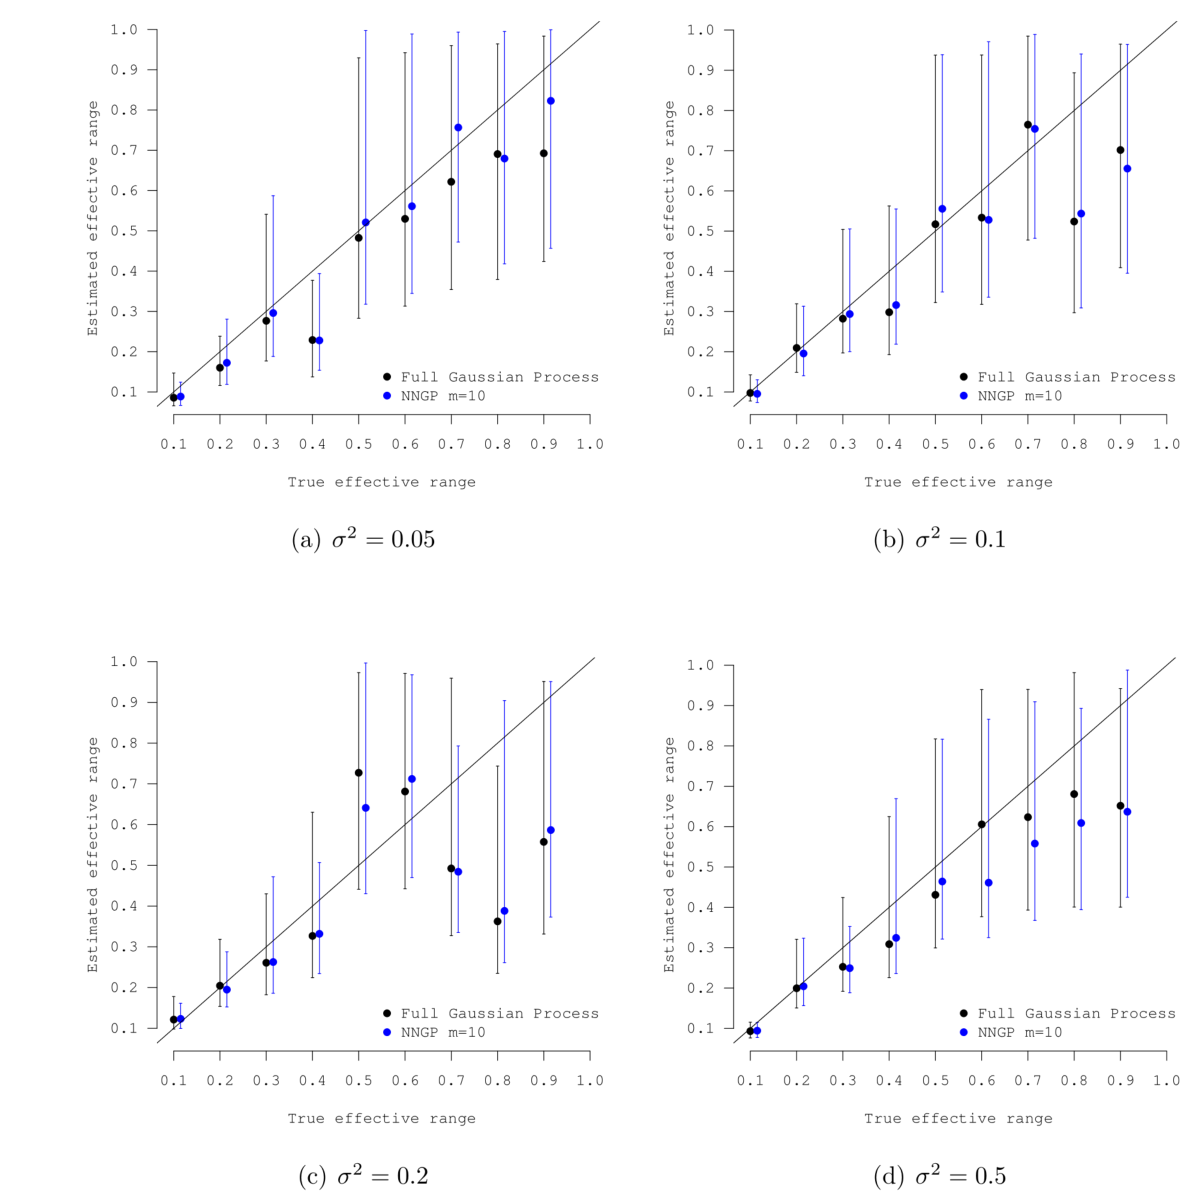
\includegraphics[width=16cm]{Figures/datta_NNGP.png} }
%\vspace{1em}
%\caption{Simulation results of \href{https://chenyw68.github.io/Literature/[2016]Hierarchical nearest-neighbor Gaussian process models for large geostatistical datasets.pdf}{\cite{datta2016hierarchical}}.}\label{fig:datta}
%\end{figure}


We considered model (\ref{model}) with $\boldsymbol{\beta X} = 0.1\boldsymbol{I}, \sigma^2 = 5, \tau^2 = 1$, and the Matern correlation function for the spatial random effects $\boldsymbol{w}$, with a constant smoothness parameter $\nu = 0.5$ and varying spatial range parameters.

Three distance criteria:
\begin{align}
D_{\mathrm{KL}}(\hat{\mathbf{\Sigma}}, \mathbf{\Sigma}) &=\frac{1}{2}\left[\operatorname{trace}\left(\hat{\mathbf{\Sigma}}^{-1} \mathbf{\Sigma}\right)- p +\log |\hat{\mathbf{\Sigma}}|-\log |\mathbf{\Sigma}|\right] \\
D_{\mathrm{B}}(\hat{\mathbf{\Sigma}}, \mathbf{\Sigma}) &=\frac{1}{2} \log |\tilde{\mathbf{\Sigma}}|-\frac{1}{4}\log | \hat{\mathbf{\Sigma}} |-\frac{1}{4} \log | \mathbf{\Sigma} |, \quad \tilde{\mathbf{\Sigma}}=[\mathbf{\Sigma}+\hat{\mathbf{\Sigma}}] / 2 \\
D_{\mathrm{F}}(\hat{\mathbf{\Sigma}}, \mathbf{\Sigma}) &=\sqrt{\operatorname{trace}\left[(\hat{\mathbf{\Sigma}}-\mathbf{\Sigma})(\hat{\mathbf{\Sigma}}-\mathbf{\Sigma})^{\prime}\right]}
\end{align}

%\begin{figure}[H]
%{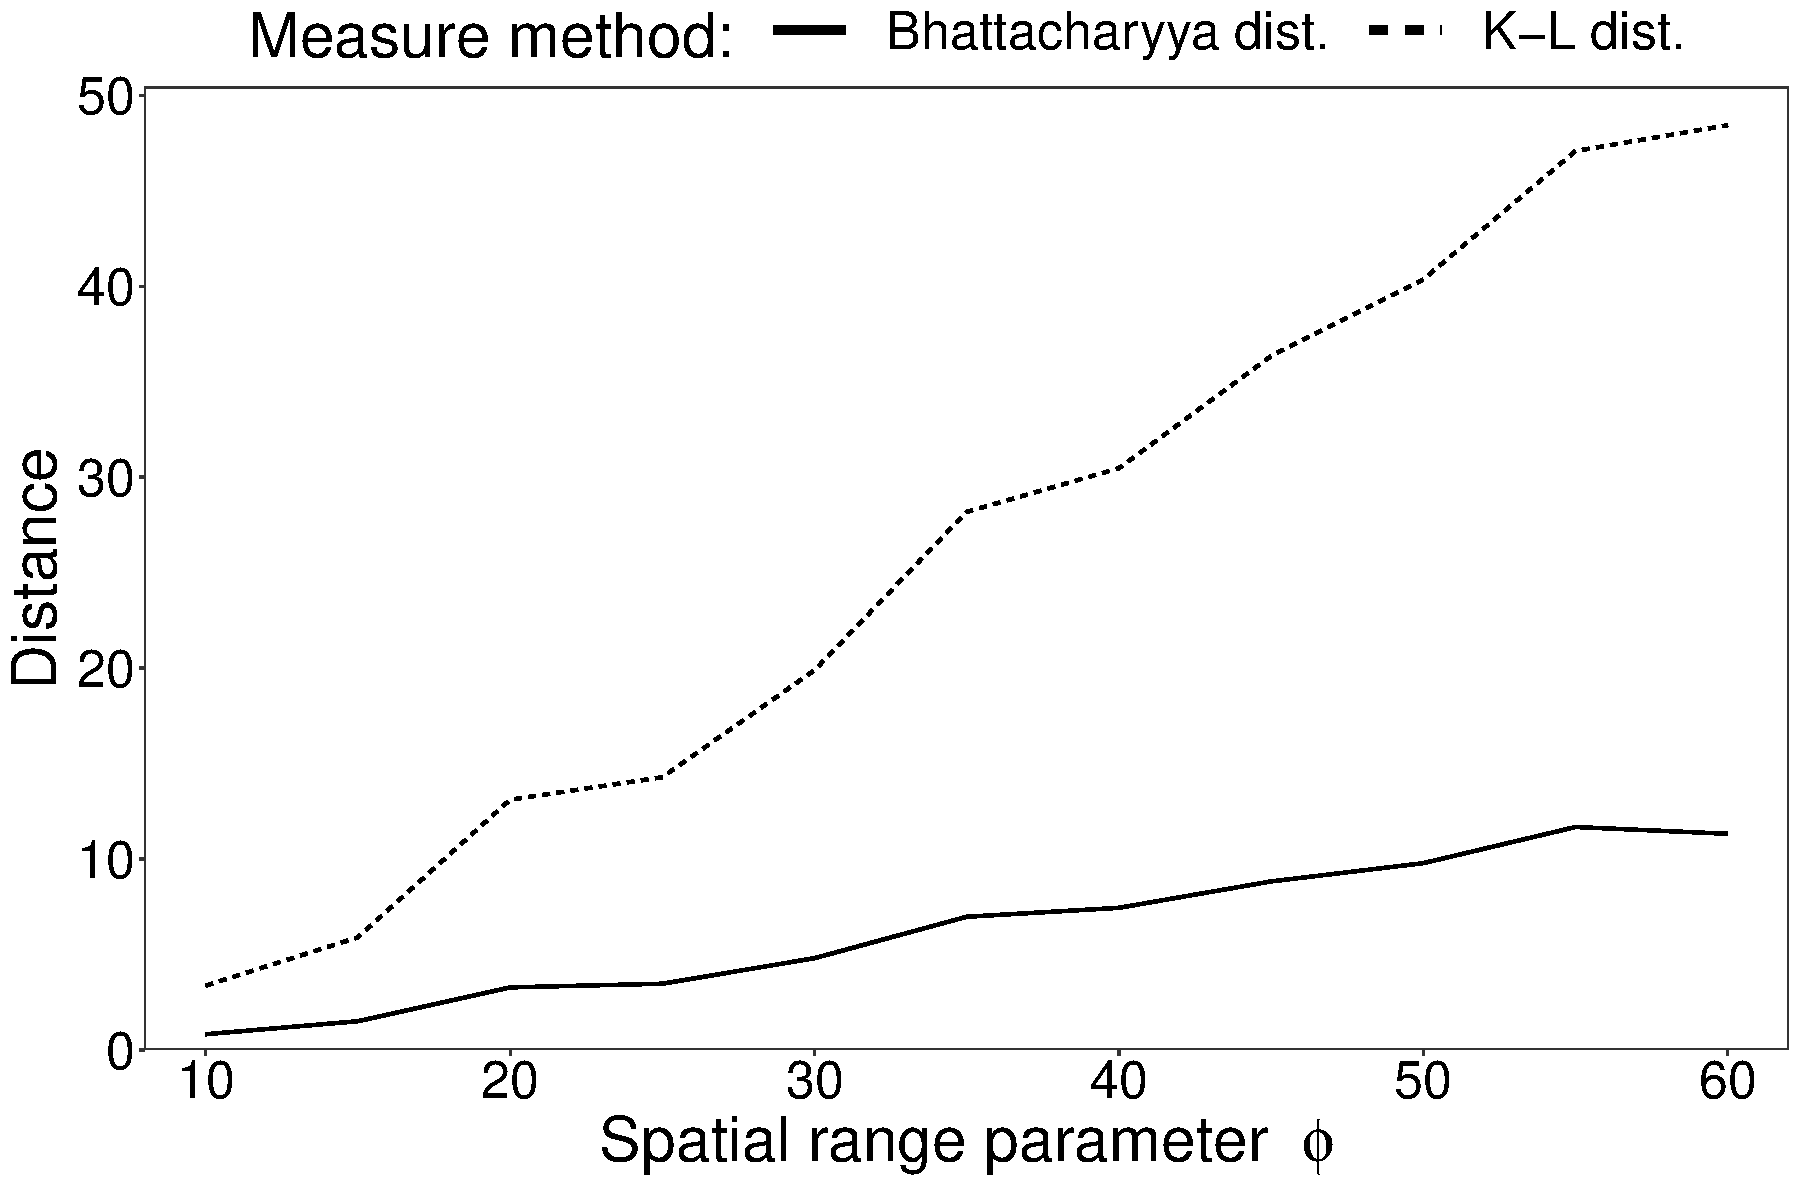
\includegraphics[width=8cm]{Figures/nnGP1.pdf} }
%{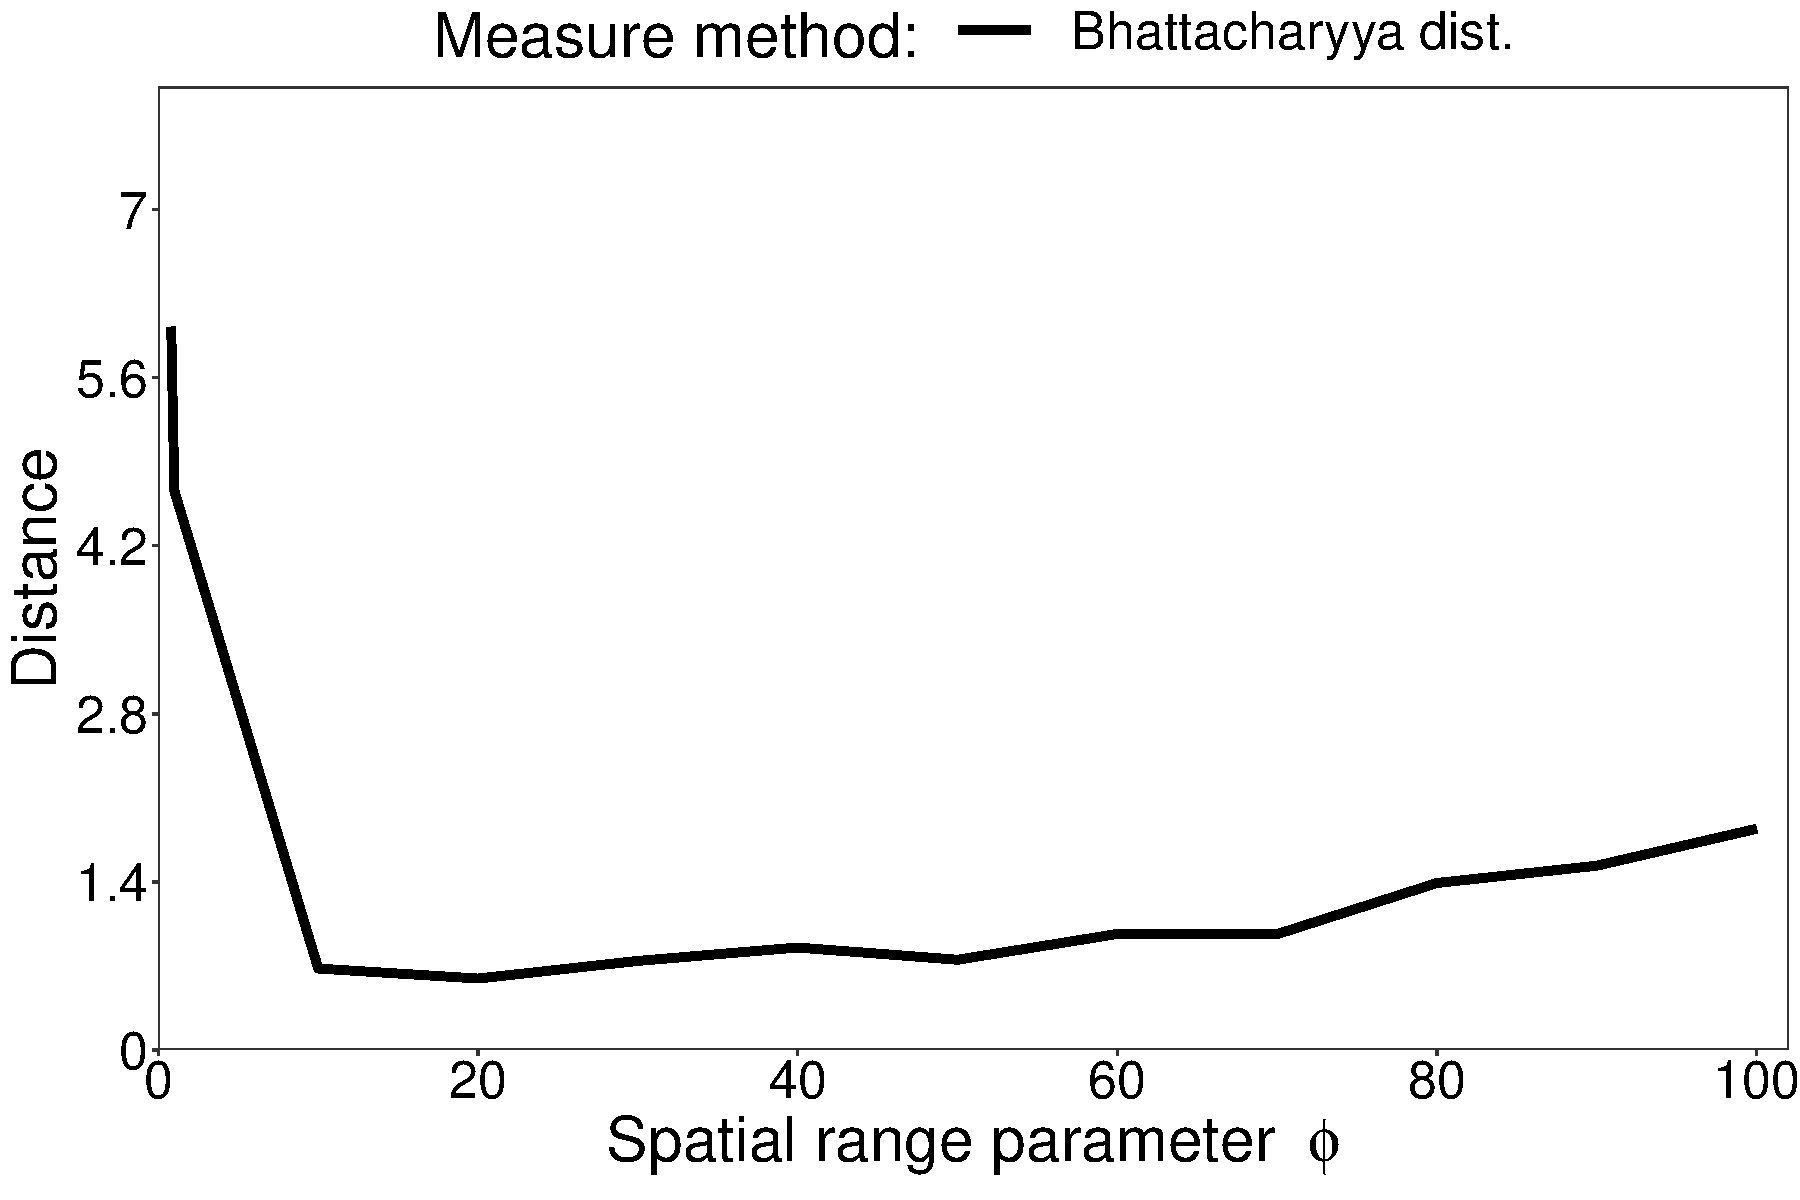
\includegraphics[width=8cm]{Figures/nnGP2.pdf} }
%{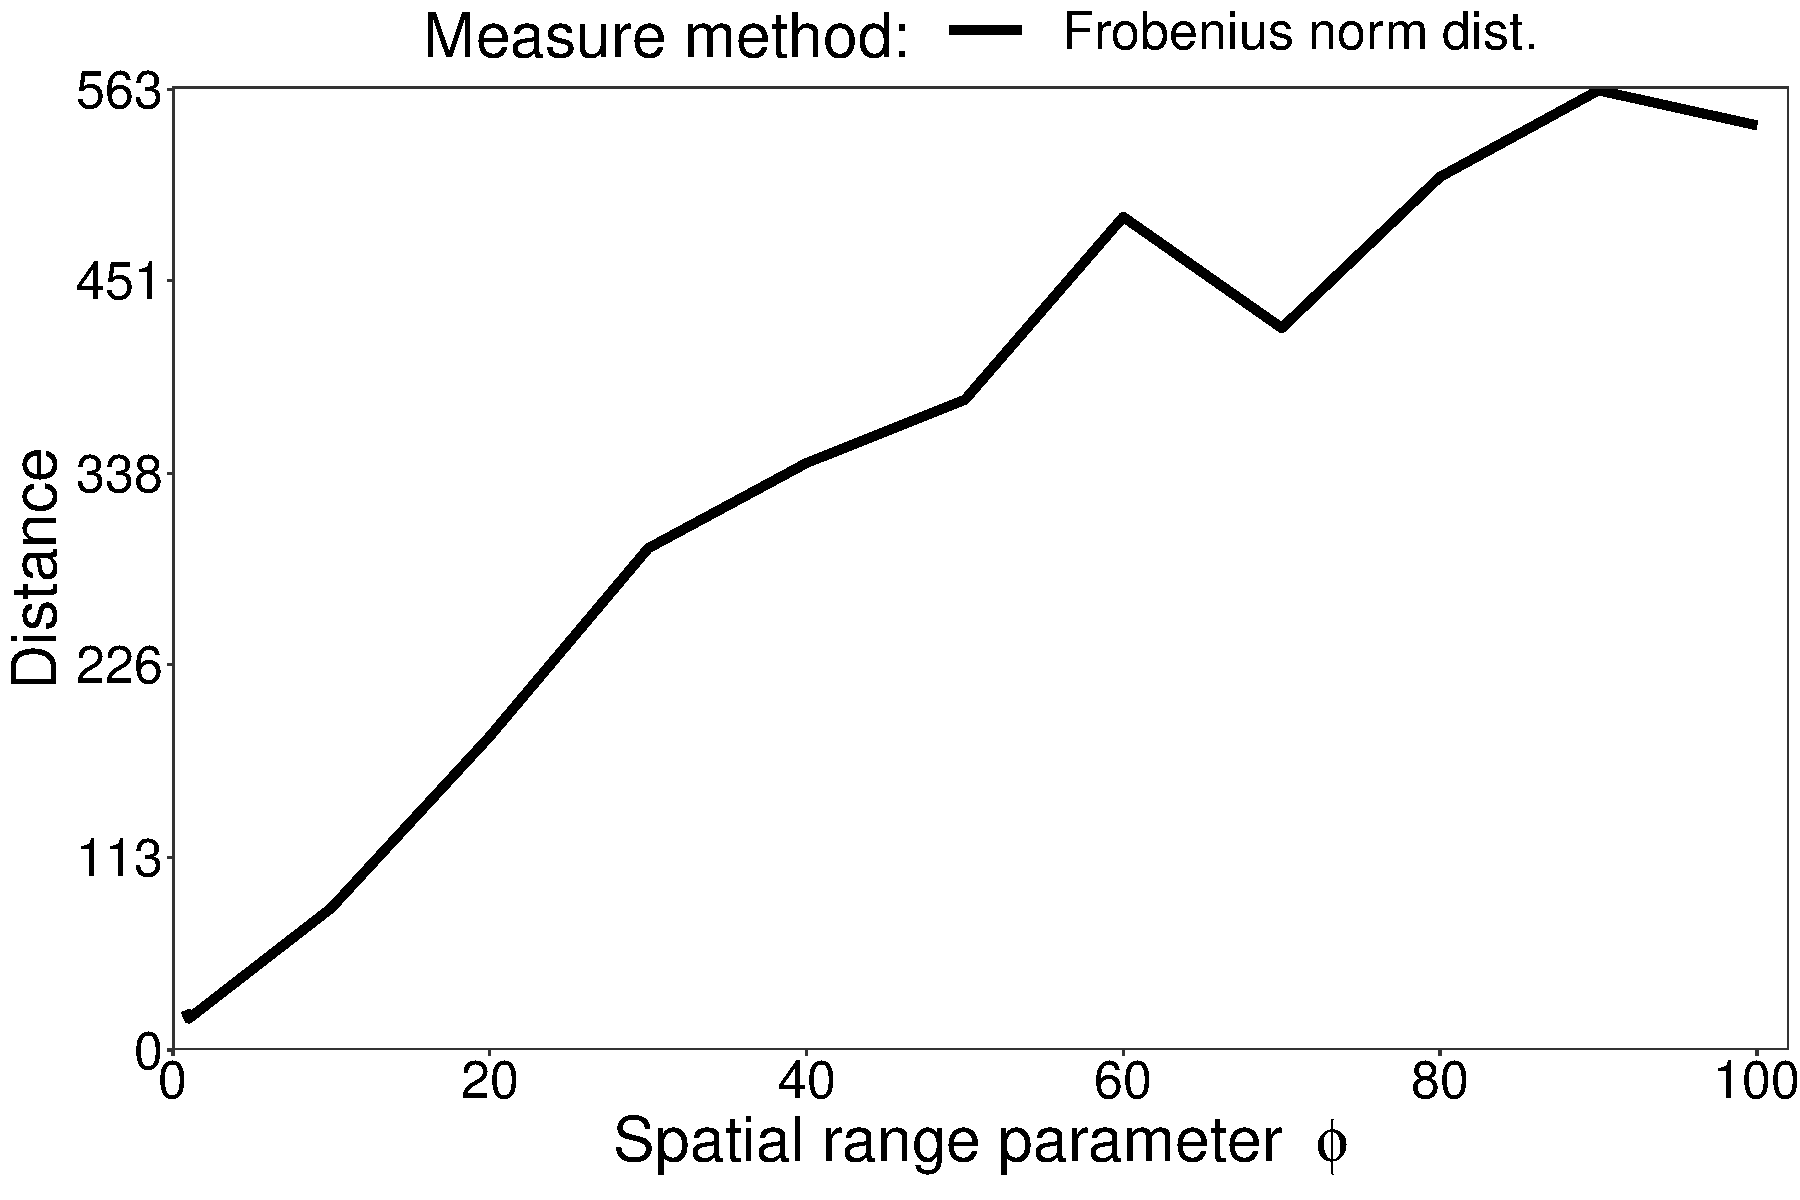
\includegraphics[width=8cm]{Figures/nnGP3.pdf} }
%\vspace{1em}
%\caption{The K-L distance, the Bhattacharyya distance and the Frobenius norm from the estimated covariance
%matrix to the true covariance matrix for the Matérn family with smoothness parameters $\nu = \frac{1}{2}$ and different spatial range parameters $\phi$. And this true covariance matrix at $500$ random locations from $[0, 100] \times [0, 100]$ was estimated by the NNGP model with $m = 20$  for 50 simulations.}\label{fig:nnGP1}
%\end{figure}
%
%\begin{figure}[H]
%{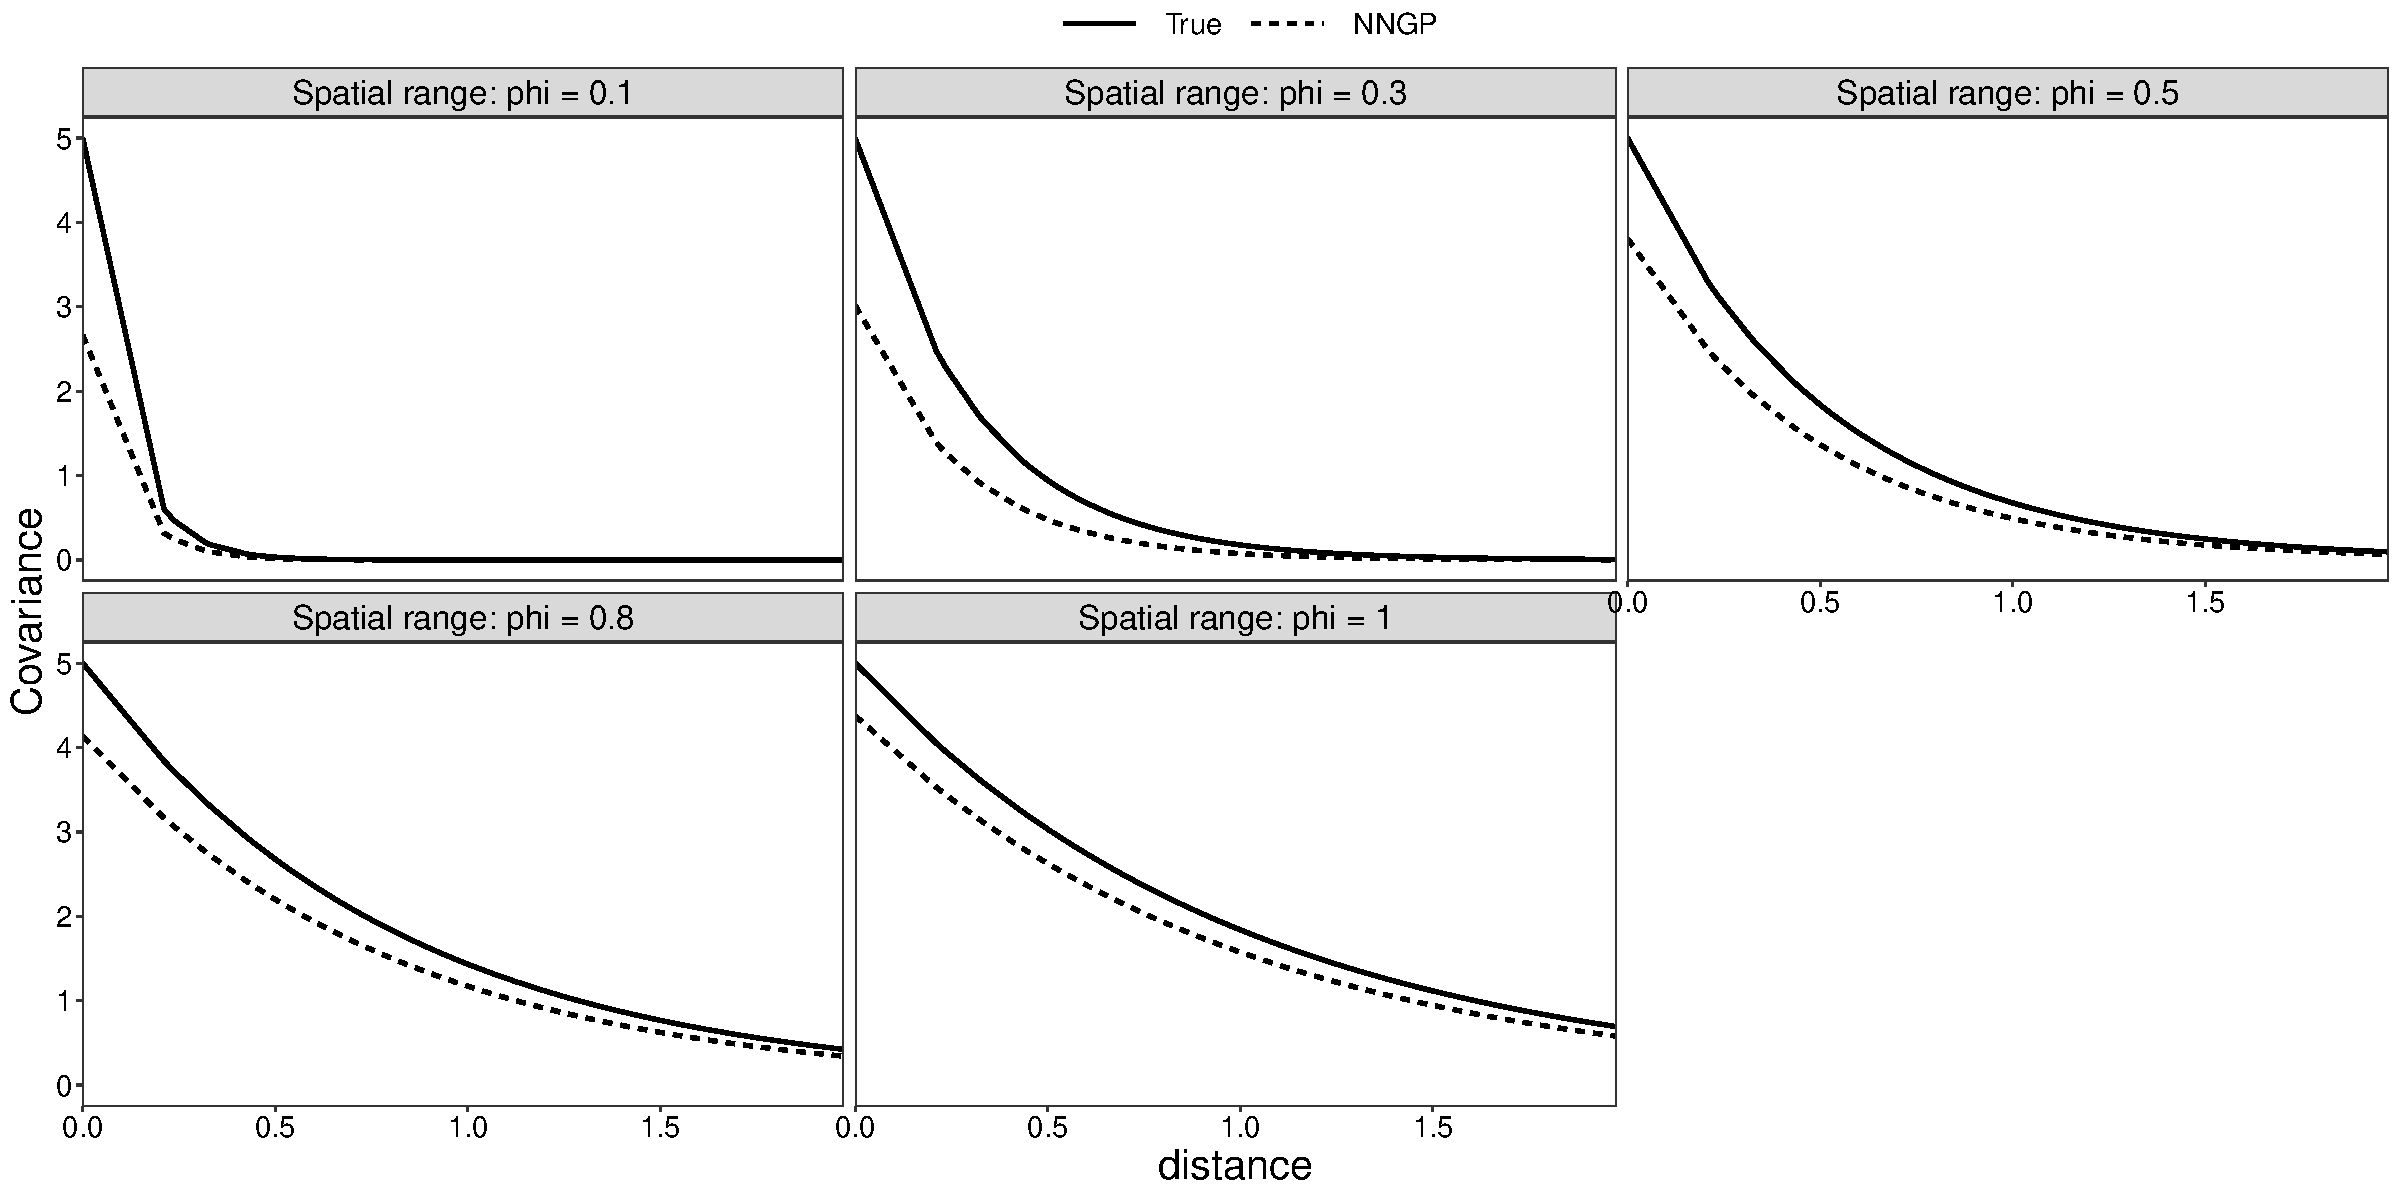
\includegraphics[width=18cm]{Figures/nnGP_Cov1.pdf} }
%{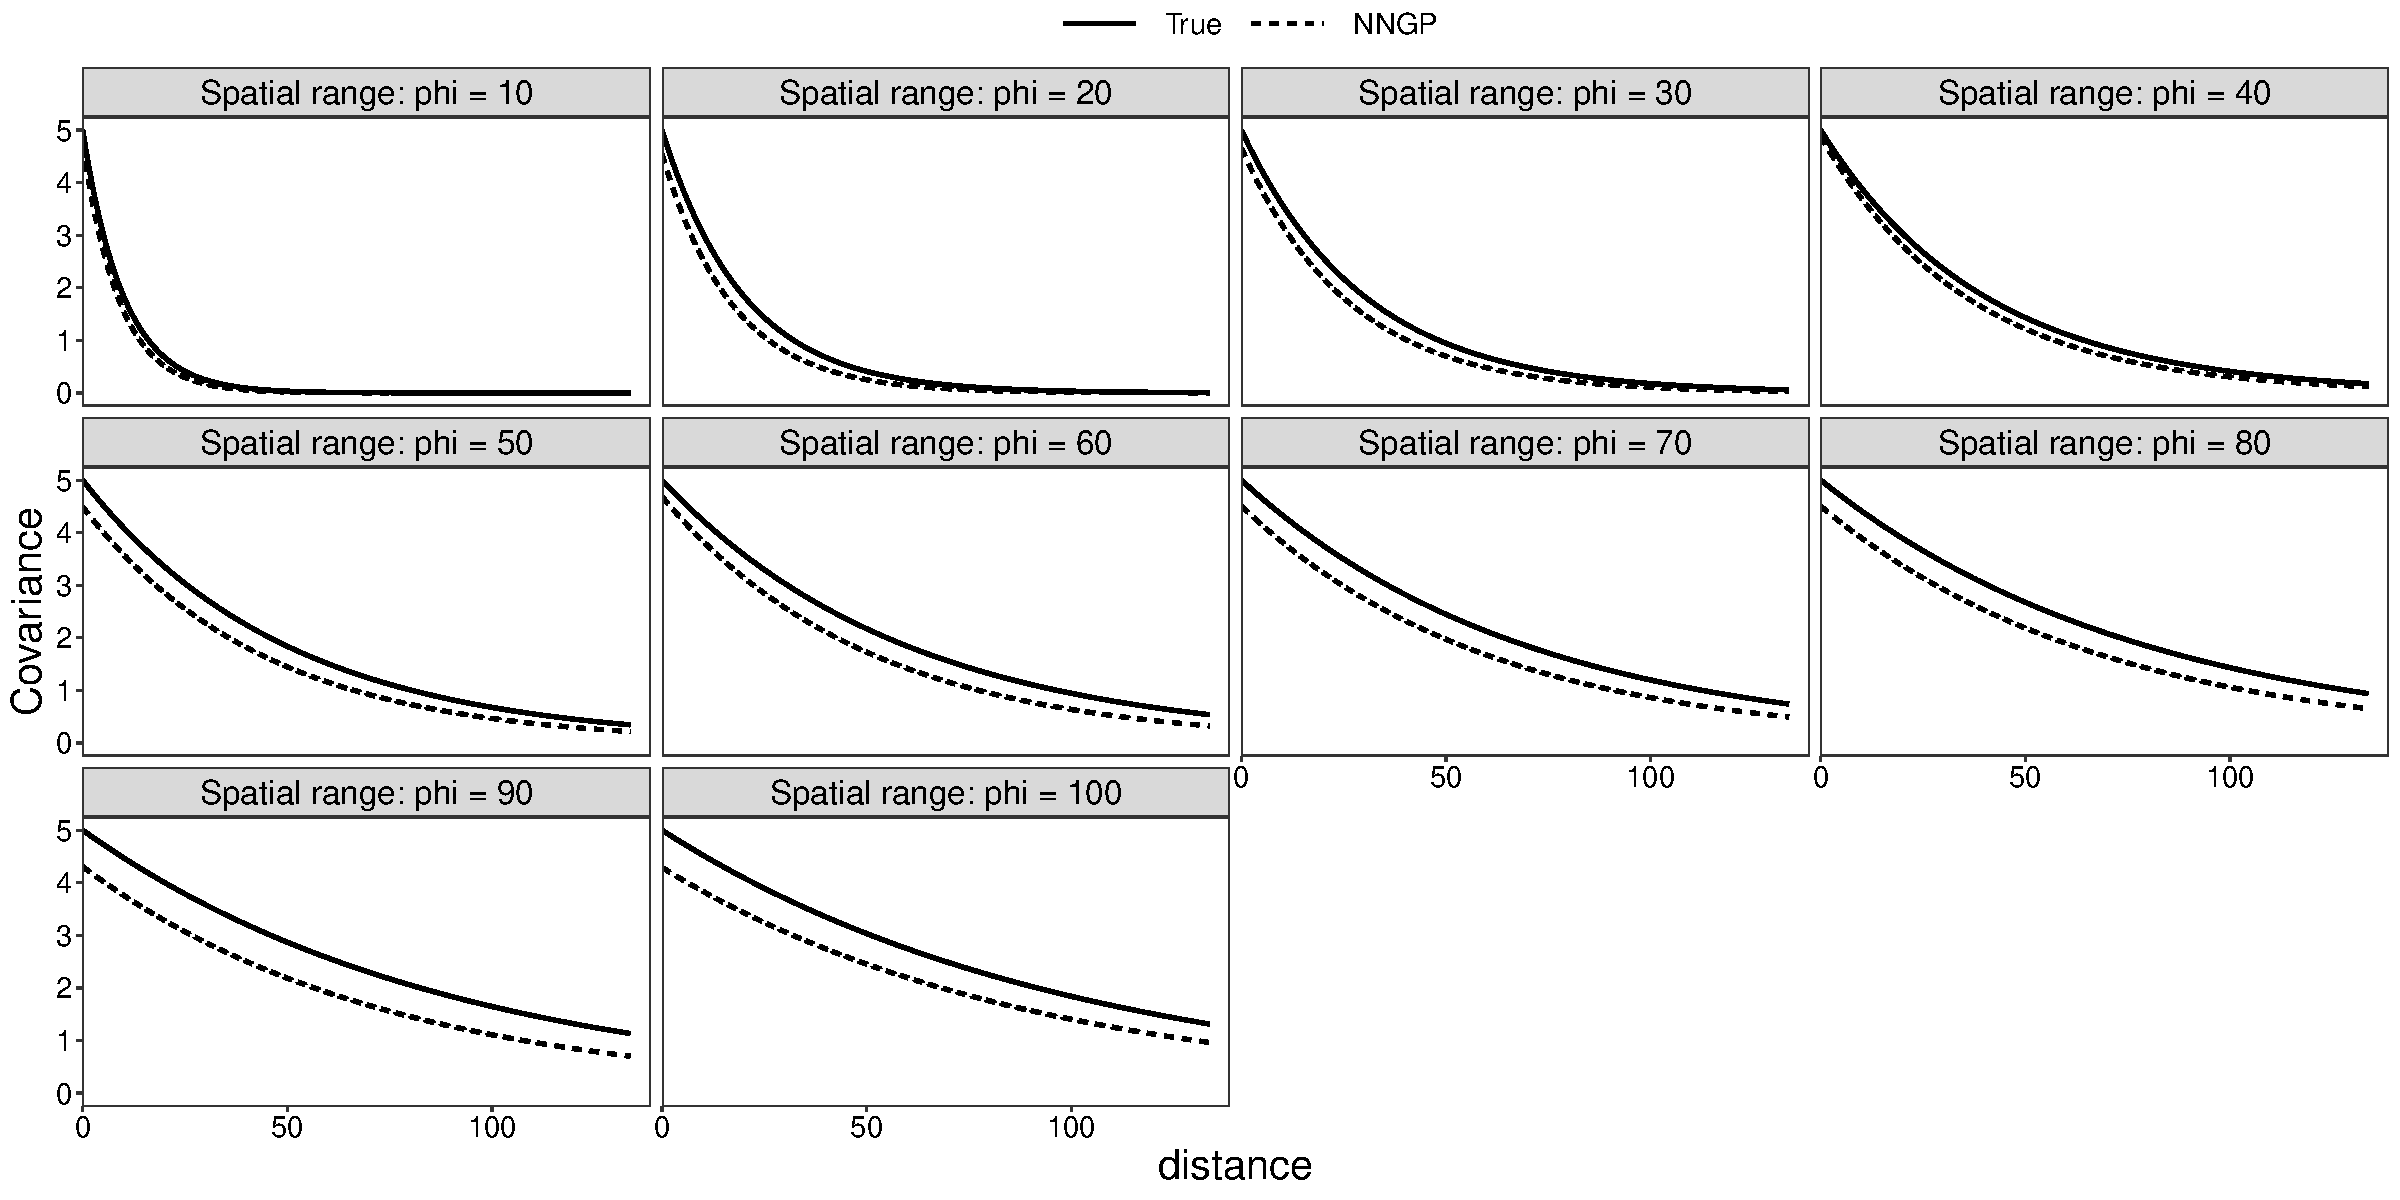
\includegraphics[width=18cm]{Figures/nnGP_Cov2.pdf} }
%\vspace{1em}
%\caption{Estimation results of covariance function corresponding to Figure \ref{fig:nnGP1}.}\label{fig:nnGP2}
%\end{figure}

Figure \ref{fig:nnGP1} and \ref{fig:nnGP2} suggest that \textbf{the large-scale spatial dependencies for a larger domain can not be well-captured} by the NNGP, and at the same time, the top two panel of Figure \ref{fig:nnGP1} show that as with predictive process model, the NNGP may also \textbf{fail to capture some local information}, that may be related to the selection of reference set.

\subsection{\textcolor[rgb]{1.00,0.00,0.50}{Improvement project}}
\begin{itemize}
 \item [1)] Ideas for Problem 1: Combing a NNGP $w(s)$ used to capture the \textcolor[rgb]{0.50,0.50,0.50}{local, small scale dependence structure} with its spatial smooth version $f(s)$ used to capture the \textcolor[rgb]{0.50,0.50,0.50}{large scale dependence structure}, for example,
\begin{equation}
\begin{aligned}
  y(s) = \boldsymbol{x}(s)\boldsymbol{\beta} + w(s) + f(s) + \epsilon(s).
\end{aligned} \label{DP1}
\end{equation}
%where $\boldsymbol{w} = \left(w(s_1), \cdots, w(s_n)\right)^\prime \sim NNGP\left(\boldsymbol{0}, \boldsymbol{\tilde{C}}_1(\cdot; \boldsymbol{\theta}_1)\right)$; by denoting $h_{k}, k = 1, \cdots, K$ as a sequence of fixed basis functions and
%let $f(s) = \sum_{k = 1}^{K}h_{k}(s)w_{k}^{\star}$ and the basis coefficients $\boldsymbol{w}^{\star} = \left(w_1^{\star}, \cdots, w_K^{\star}\right)^\prime \sim NNGP\left(\boldsymbol{0}, \boldsymbol{\tilde{C}}_2(\cdot; \boldsymbol{\theta}_2)\right)$,
%%\textbf{automatically chosen by a given covariance function}, i.e. $\tilde{c}^\prime(k, \mathcal{N}(k))\boldsymbol{\tilde{C}}_2^{-1}\left(\mathcal{N}(k), \mathcal{N}(k)\right)$;
%$\boldsymbol{\epsilon} = \left(\epsilon(s_1), \cdots, \epsilon(s_n)\right)^\prime \sim N(\boldsymbol{0}, \tau^2\boldsymbol{I})$. And thereby, we have
%\begin{equation}
%\begin{aligned}
%\boldsymbol{y} \sim GP\left(\boldsymbol{0}, \boldsymbol{\Sigma}(\cdot; \boldsymbol{\theta})\right)
%\end{aligned} \label{DP1}
%\end{equation}
%where $\boldsymbol{\Sigma}(\cdot; \boldsymbol{\theta}) = \boldsymbol{\tilde{C}}_1(\cdot; \boldsymbol{\theta}_1) +
%\boldsymbol{H}\boldsymbol{\tilde{C}}_2(\cdot; \boldsymbol{\theta}_1)\boldsymbol{H}^\prime + \tau^2\boldsymbol{I}.$
%
%Let $\boldsymbol{A} = \boldsymbol{\tilde{C}}_1 + \tau^2\boldsymbol{I}$, and by applying the Sherman-Woodbury-Morrison formula for inverse matrices, we obtain:
%\begin{equation}
%\begin{aligned}
%  \boldsymbol{\Sigma}^{-1} = & \boldsymbol{A}^{-1} - \boldsymbol{A}^{-1}\boldsymbol{H}
%  \left(\boldsymbol{\tilde{C}}_2^{-1} + \boldsymbol{H}^\prime\boldsymbol{A}^{-1}\boldsymbol{H}\right)^{-1}\boldsymbol{H}^\prime\boldsymbol{A}^{-1}.
%\end{aligned}
%\end{equation}
%On the other hand, the determinant can be computed using
%\begin{equation}
%\begin{aligned}
%  \text{det}\{\boldsymbol{\Sigma}\} = &  \text{det}\{\boldsymbol{\tilde{C}}_2^{-1} + + \boldsymbol{H}^\prime\boldsymbol{A}^{-1}\boldsymbol{H}\}\text{det}\{\boldsymbol{\tilde{C}}_2\}\text{det}\{\boldsymbol{A}\}.
%\end{aligned}
%\end{equation}
Denote the reference set as $\boldsymbol{S} = \{s_j^{\star}: j = 1, \cdots, K\}$ determined through the grid of the domain and $w(s_j^{\star})$ as $w^{\star}_j$. Assume that $\boldsymbol{w}^{\star} = \left(w_1^{\star}, \cdots, w_K^{\star}\right)^\prime \sim NNGP\left(\boldsymbol{0}, \boldsymbol{{C}^{\star}}(\cdot; \boldsymbol{\theta})\right)$ and $h_{k}, k = 1, \cdots, K$ is a sequence of fixed basis functions, and the $w(s)$ and $f(s)$ are then constructed as follows:
\begin{equation}
\begin{aligned}
w(s) = \boldsymbol{b}^\prime_s \boldsymbol{w}^{\star} \label{Sm1}
\end{aligned}
\end{equation}
and
\begin{equation}
\begin{aligned}
f(s) = \sum_{k = 1}^{K}h_{k}(s)w_{k}^{\star} = \boldsymbol{h}^\prime(s) \boldsymbol{w}^{\star}\label{Sm2}
\end{aligned}
\end{equation}
where
\begin{equation}
\boldsymbol{b}^\prime_s = \left\{
\begin{aligned}
&\left(\mathbbm{1}\left(s = 1\right), \cdots, \mathbbm{1}\left(s = k\right), \cdots, \mathbbm{1}\left(s = K\right) \right), \text{ if } s \in \boldsymbol{S}\\ &
\mathcal{G}\left(s; \boldsymbol{c}_{s, N(s)} \boldsymbol{C}_{N(s)}^{-1}\right), \text{ otherwise }
\end{aligned}
\right.\label{Sm3}
\end{equation}
%and $d_{s, k} = \mathbbm{1}\left(s \in \boldsymbol{S}\right) \mathbbm{1}\left(s=k\right) + \mathbbm{1}\left(s \notin \boldsymbol{S}\right)\mathbbm{1}\left(s \neq k\right)\mathcal{G}\left(s; \boldsymbol{c}_{s, N(s)}^\prime \boldsymbol{C}_{N(s)}^{-1}\right)$,
and the function of $\mathcal{G}(s; \boldsymbol{a}_s)$ is to expand the vector $\boldsymbol{a}_s$ from the low-dimension to high-dimension (e.g., from $m$ to $K$) with  according to the index of neighbor set for the location $s$, and then to derive a vector $\boldsymbol{b}_s$ where $\boldsymbol{b}_s(j) = \boldsymbol{a}_s(j)$ if $j$ is the neighbor of location $s$ corresponding to $w_j^{\star}$, 0 otherwise.

In terms of matrix-vector representation, obtaining
\begin{equation}
\begin{aligned}
\boldsymbol{y} = \boldsymbol{X}\boldsymbol{\beta} + \left(\boldsymbol{B} + \boldsymbol{H}\right)\boldsymbol{w}^{\star} + \epsilon(s)
\end{aligned} \label{DP12}
\end{equation}
where $\boldsymbol{B} = \left(\boldsymbol{b}^\prime_1, \dots, \boldsymbol{b}^\prime_n\right)^\prime$ and $\boldsymbol{H} = \left(\boldsymbol{h}^\prime(1), \dots, \boldsymbol{h}^\prime(n)\right)^\prime$. And according to the assumptions previously mentioned in the model, we know that
\begin{equation}
\begin{aligned}
\boldsymbol{y} \sim GP\left(\boldsymbol{X}\boldsymbol{\beta}, \boldsymbol{\Sigma}(\cdot; \boldsymbol{\theta})\right)
\end{aligned} \label{DP13}
\end{equation}
where $\boldsymbol{\Sigma}(\cdot; \boldsymbol{\theta}) = \left(\boldsymbol{B} + \boldsymbol{H}\right) \boldsymbol{{C}^{\star}}(\cdot; \boldsymbol{\theta})\left(\boldsymbol{B} + \boldsymbol{H}\right)^\prime + \tau^2\boldsymbol{I}.$

Let $\boldsymbol{U} = \boldsymbol{B} + \boldsymbol{H}$, and by applying the Sherman-Woodbury-Morrison formula for inverse matrices (as $n \gg K$), we have
\begin{equation}
\begin{aligned}
  \boldsymbol{\Sigma}^{-1} = & \frac{1}{\tau^2}\boldsymbol{I} - \frac{1}{\tau^2}\boldsymbol{U}
  \left(\tau^2\boldsymbol{{{C}^{\star}}^{-1}} + \boldsymbol{U}^\prime\boldsymbol{U}\right)^{-1}\boldsymbol{U}^\prime.
\end{aligned} \label{Sov}
\end{equation}

On the other hand, the determinant can be computed using
\begin{equation}
\begin{aligned}
  \text{det}\{\boldsymbol{\Sigma}\} = &  \tau^{2(n - K)} \frac{\text{det}\{\tau^2\boldsymbol{{{C}^{\star}}^{-1}} +  \boldsymbol{U}^\prime\boldsymbol{U}\}}{\text{det}\{\boldsymbol{{{C}^{\star}}^{-1}}\}}.
\end{aligned}\label{Det}
\end{equation}
Recall that $\boldsymbol{{{C}^{\star}}^{-1}}$ is a sparse precision matrix with at most $Km(m + 1)/2$ nonzero entries, thereby, (\ref{Sov}) and (\ref{Det}) can facilitate computations.

With customary prior specifications, we obtain the joint distribution:%\left(\mathbf{D + H}\right)\left({s}_{i}\right)\mathbf{w}, \tau^2\right)
\begin{equation}
\begin{aligned}
& \prod_{i=1}^{n} N\left(\mathbf{y}\left({s}_{i}\right) \mid \mathbf{x}\left({s}_{i}\right) \boldsymbol{\beta}+
w\left(s_i\right) + \mathbf{h}^\prime(s_i)\mathbf{w}^{\star}\right) \times N\left(\boldsymbol{w}_{U} \mid \mathbf{b}_{U}\mathbf{w}^{\star}, \boldsymbol{V}_{U}\right) \times \\ &
N\left(\mathbf{w}^{\star} \mid \boldsymbol{0}, {\mathbf{C}}^{\star}\right) \times N\left(\boldsymbol{\beta} \mid \boldsymbol{\mu}_{\beta}, \mathbf{V}_{\beta}\right) \times  \prod_{j=1}^{l} I G\left(\tau_{j}^{2} \mid a_{\tau_{j}}, b_{\tau_{j}}\right) \times p(\boldsymbol{\theta})
\end{aligned}
\end{equation}

\begin{itemize}
 \item [\textbf{Step1}]
\(\operatorname{Set} \pi(\boldsymbol{\beta})=N\left(\boldsymbol{\mu}_\beta, \boldsymbol{D}_\beta\right),\)
then
\(p\left(\boldsymbol{\beta} | \boldsymbol{y}, \boldsymbol{w}^{\star}, \boldsymbol{\theta}, \tau^{2}\right)=N(\boldsymbol{D}^{\star}_\beta \boldsymbol{\eta}^{\star}_\beta, \boldsymbol{D}^{\star}_\beta),\)
where \begin{equation}
\boldsymbol{D}^{\star}_\beta=\left(\frac{\boldsymbol{X}^{\prime} \boldsymbol{X}}{\tau^{2}}+\boldsymbol{D}_{\beta}^{-1}\right)^{-1} ; \boldsymbol{\eta}^{\star}_\beta=\frac{\boldsymbol{X}^{\prime}\left(\boldsymbol{y}-\left(\boldsymbol{B} + \boldsymbol{H}\right)\boldsymbol{w}^{\star}\right)}{\tau^{2}}+\boldsymbol{D}_{\beta}^{-1} \boldsymbol{\mu}_\beta \label{Eq:Post_Beta_Dis}
\end{equation}

\begin{figure}[H]
\centering{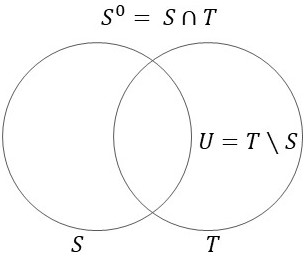
\includegraphics[width=4cm]{Figures/Set} }
\vspace{1em}
\caption{Representation of several sets.}\label{fig:set}
\end{figure}

 \item [\textbf{Step2}] 
Set \(\pi(\boldsymbol{w})=N\left(0, \boldsymbol{C}\left(\cdot; \boldsymbol{\theta}\right)\right).\)

then \(p(w_i | y\left(s_i\right), \boldsymbol{x}\left(s_i\right)\boldsymbol{\beta}, \boldsymbol{\theta})\) is
again of the form \(N(\sigma_i^2 \eta_i, \sigma_i^2),\)

\textcolor[rgb]{0.60,0.80,0.20}{For $i \in \boldsymbol{U}$}, $i = r, \cdots, n$, where
\begin{equation}
\sigma_i^2 = \left(\frac{1}{\tau^2} + \frac{1}{v_i^2} \right)^{-1} ; 
\eta_i = \frac{y\left(s_i\right) - \boldsymbol{x}\left(s_i\right)\boldsymbol{\beta} - \boldsymbol{H}\boldsymbol{w}^{\star}}{\tau^{2}} +  \frac{c_{s_i} \boldsymbol{w}^{\star}_{N(s_i)}}{v_i^2}
 \label{Eq:Post_W_Dis}
\end{equation}

\textcolor[rgb]{0.60,0.80,0.20}{For $i \in \boldsymbol{S}$}, $i = 1, \cdots, K$,  let $U(s_i) = \{j \in \boldsymbol{S} \cup \boldsymbol{T}\mid s_i \in N(j)\},$ $\boldsymbol{c}_{s_i} = \boldsymbol{c}_{\left(s_i, N(s_i)\right)}\boldsymbol{C}_{N(s_i)}^{-1}$, $v_i^2 = c(s_i, s_i) - \boldsymbol{c}_{\left(s_i, N(s_i)\right)}\boldsymbol{C}_{N(s_i)}^{-1}\boldsymbol{c}_{\left(N(s_i), s_i\right)}$ and $\boldsymbol{S}^{o}$ represents set of some knots with observed values. 

For every $j \in U(s_i)$, define $a_{j}(s_i) = \left(w_j - \sum_{s \in N(j), s \neq s_i}{c_{j}(s)w^{\star}(s)}\right)$, where $c_{j}(s)$  is the element from $\boldsymbol{c}_{j}$ that corresponds to the knot $s$.
Consider $\boldsymbol{p\left[y_i\mid w_i, \cdot\right]p\left[w_i\mid w_{N(i)}\right]p\left[w_j\mid w_{N(j), i \in N(j)}\right]}$, we have
\begin{equation}
\begin{aligned}
&\sigma_i^2 = \left(\frac{\left(1 + h_i(s_i)\right)^2}{\tau^2}\mathbbm{1}\left(s_i \in \boldsymbol{S}^{o}\right) + \frac{1}{v_i^2} + 
\sum_{j \in U(s_i)}\frac{c_{j}^2(s_i)}{v_j^2} \right)^{-1}, \\&
\eta_i = \frac{\left(1 + h_i(s_i)\right)\left(y\left(s_i\right) - \boldsymbol{x}\left(s_i\right)\boldsymbol{\beta} - \sum_{k \neq i}^{K}h_k(s_i)w_k^{\star}\right)}{\tau^{2}}\mathbbm{1}\left(s_i \in \boldsymbol{S}^{o}\right)\\& ~~~~~~~ + \frac{c_{s_i} \boldsymbol{w}_{N(s_i)}^{\star}}{v_i^2} + \sum_{j \in U(s_i)}\frac{a_{j}(s_i)c_j(s_i)}{v_j^2}.
\end{aligned}
 \label{Eq:Post_W_Dis}
\end{equation}

\item [\textbf{Step3}] Furthermore, set
\(\pi\left(\tau^{2}\right)=I G\left(a_{\tau}, b_{\tau}\right), \pi\left(\sigma^{2}\right)=I G\left(a_{\sigma}, b_{\sigma}\right),\)
respectively, then \begin{equation}
p\left(\tau^{2} | \boldsymbol{y}, \boldsymbol{X}, \boldsymbol{\beta}, \boldsymbol{w}\right)=I G\left(a_{\tau}+\frac{n}{2}, b_{\tau}+\frac{(\boldsymbol{y}-\boldsymbol{X} \boldsymbol{\beta}-\boldsymbol{w})^{\prime}(\boldsymbol{y}-\boldsymbol{X} \boldsymbol{\beta}-\boldsymbol{w})}{2}\right)
\end{equation}

\begin{equation}
p\left(\sigma^{2} | \phi, \boldsymbol{w}\right)=I G\left(a_{\sigma}+\frac{n}{2}, b_{\sigma}+\frac{\boldsymbol{w}^{\prime} \boldsymbol{H}^{-1}(\phi) \boldsymbol{w}}{2}\right)
\end{equation}

 \item [\textbf{Step4}] However, no closed form is available for
\(p\left(\phi | \boldsymbol{w}, \sigma^{2}\right)\) as follow
\begin{equation}
p\left(\phi | \boldsymbol{w}, \sigma^{2}\right) \propto \pi(\phi) \exp \left(-\frac{\boldsymbol{w}^{\prime} \boldsymbol{H}^{-1}(\phi) \boldsymbol{w}}{2\sigma^2}\right)
\end{equation} Except \(\phi^{\prime}\) s sample, the other can be
sampled by Gibbs sampler, while the former can be taken by Metropolis
algorithm or slice sampling.
\end{itemize}



 \item [2)] Ideas for Problem 2: Similar to \href{https://chenyw68.github.io/Literature/[2012]A full scale approximation of covariance functions for large spatial data sets.pdf}{\cite{sang2012full}},
\begin{equation}
    \begin{aligned}
       y(s) = w_l(s) + w_s(s) + \epsilon(s)
    \end{aligned} \label{DP1}
\end{equation}
where $w_l$ is a NNGP and $w_s$ is a residual process with covariance function constrained by tapered function.
 \item [3)] A more thorough solution for both problems: Similar to LatticeKrig, to build a multi-resolution NNGP approximation, i.e.,
 \begin{equation}
\begin{aligned}
y(s) = \sum_{r = 1}^{R}\sum_{k = 1}^{K_r}h_{ri}(s)w_{rk}^{\star}  + \epsilon(s)
\end{aligned} \label{DP1}
\end{equation}
where $\boldsymbol{w}_r^{\star} = \left(w_{r, 1}^{\star}, \cdots, w_{r, K_r}^{\star}\right)^\prime \sim NNGP\left(\boldsymbol{0}, \boldsymbol{\tilde{C}}_r(\cdot; \boldsymbol{\theta}_r)\right)$.
\end{itemize}


some other websites: \href{http://www.randomservices.org/random/index.html}{Probability, Mathematical Statistics, Stochastic Processes}
%----------------------------------------------------------------------------------------
%\bibliographystyle{achemso}
\bibliography{summary_spatial}
\end{document} 